%% (Master) Thesis template
% Template version used: v1.4
%
% Largely adapted from Adrian Nievergelt's template for the ADPS
% (lecture notes) project.


%% We use the memoir class because it offers a many easy to use features.
\documentclass[11pt,a4paper,titlepage]{memoir}

%% Packages
%% ========

%% LaTeX Font encoding -- DO NOT CHANGE
\usepackage[OT1]{fontenc}

%% Babel provides support for languages.  'english' uses British
%% English hyphenation and text snippets like "Figure" and
%% "Theorem". Use the option 'ngerman' if your document is in German.
%% Use 'american' for American English.  Note that if you change this,
%% the next LaTeX run may show spurious errors.  Simply run it again.
%% If they persist, remove the .aux file and try again.
\usepackage[english]{babel}

%% Input encoding 'utf8'. In some cases you might need 'utf8x' for
%% extra symbols. Not all editors, especially on Windows, are UTF-8
%% capable, so you may want to use 'latin1' instead.
\usepackage[utf8]{inputenc}

%% This changes default fonts for both text and math mode to use Herman Zapfs
%% excellent Palatino font.  Do not change this.
\usepackage[sc]{mathpazo}

%% The AMS-LaTeX extensions for mathematical typesetting.  Do not
%% remove.
\usepackage{amsmath,amssymb,amsfonts,mathrsfs}

%% NTheorem is a reimplementation of the AMS Theorem package. This
%% will allow us to typeset theorems like examples, proofs and
%% similar.  Do not remove.
%% NOTE: Must be loaded AFTER amsmath, or the \qed placement will
%% break
\usepackage[amsmath,thmmarks]{ntheorem}

%% LaTeX' own graphics handling
\usepackage{graphicx}

%% We unfortunately need this for the Rules chapter.  Remove it
%% afterwards; or at least NEVER use its underlining features.
\usepackage{soul}

%% This allows you to add .pdf files. It is used to add the
%% declaration of originality.
\usepackage{pdfpages}

%% Some more packages that you may want to use.  Have a look at the
%% file, and consult the package docs for each.
%% See the TeXed file for more explanations

%% [OPT] Multi-rowed cells in tabulars
%\usepackage{multirow}

%% [REC] Intelligent cross reference package. This allows for nice
%% combined references that include the reference and a hint to where
%% to look for it.
\usepackage{varioref}

%% [OPT] Easily changeable quotes with \enquote{Text}
%\usepackage[german=swiss]{csquotes}

%% [REC] Format dates and time depending on locale
\usepackage{datetime}

%% [OPT] Provides a \cancel{} command to stroke through mathematics.
%\usepackage{cancel}

%% [NEED] This allows for additional typesetting tools in mathmode.
%% See its excellent documentation.
\usepackage{mathtools}

%% [ADV] Conditional commands
%\usepackage{ifthen}

%% [OPT] Manual large braces or other delimiters.
%\usepackage{bigdelim, bigstrut}

%% [REC] Alternate vector arrows. Use the command \vv{} to get scaled
%% vector arrows.
\usepackage[h]{esvect}

%% [NEED] Some extensions to tabulars and array environments.
\usepackage{array}

%% [OPT] Postscript support via pstricks graphics package. Very
%% diverse applications.
%\usepackage{pstricks,pst-all}

%% [?] This seems to allow us to define some additional counters.
%\usepackage{etex}

%% [ADV] XY-Pic to typeset some matrix-style graphics
%\usepackage[all]{xy}

%% [OPT] This is needed to generate an index at the end of the
%% document.
%\usepackage{makeidx}

%% [OPT] Fancy package for source code listings.  The template text
%% needs it for some LaTeX snippets; remove/adapt the \lstset when you
%% remove the template content.
\usepackage{listings}
\lstset{language=TeX,basicstyle={\normalfont\ttfamily}}

%% [REC] Fancy character protrusion.  Must be loaded after all fonts.
\usepackage[activate]{pdfcprot}

%% [REC] Nicer tables.  Read the excellent documentation.
\usepackage{booktabs}


%% Our layout configuration.  DO NOT CHANGE.
%% Memoir layout setup

%% NOTE: You are strongly advised not to change any of them unless you
%% know what you are doing.  These settings strongly interact in the
%% final look of the document.

% Dependencies
\usepackage{ETHlogo}

% Turn extra space before chapter headings off.
\setlength{\beforechapskip}{0pt}

\nonzeroparskip
\parindent=0pt
\defaultlists

% Chapter style redefinition
\makeatletter

\if@twoside
  \pagestyle{Ruled}
  \copypagestyle{chapter}{Ruled}
\else
  \pagestyle{ruled}
  \copypagestyle{chapter}{ruled}
\fi
\makeoddhead{chapter}{}{}{}
\makeevenhead{chapter}{}{}{}
\makeheadrule{chapter}{\textwidth}{0pt}
\copypagestyle{abstract}{empty}

\makechapterstyle{bianchimod}{%
  \chapterstyle{default}
  \renewcommand*{\chapnamefont}{\normalfont\Large\sffamily}
  \renewcommand*{\chapnumfont}{\normalfont\Large\sffamily}
  \renewcommand*{\printchaptername}{%
    \chapnamefont\centering\@chapapp}
  \renewcommand*{\printchapternum}{\chapnumfont {\thechapter}}
  \renewcommand*{\chaptitlefont}{\normalfont\huge\sffamily}
  \renewcommand*{\printchaptertitle}[1]{%
    \hrule\vskip\onelineskip \centering \chaptitlefont\textbf{\vphantom{gyM}##1}\par}
  \renewcommand*{\afterchaptertitle}{\vskip\onelineskip \hrule\vskip
    \afterchapskip}
  \renewcommand*{\printchapternonum}{%
    \vphantom{\chapnumfont {9}}\afterchapternum}}

% Use the newly defined style
\chapterstyle{bianchimod}

\setsecheadstyle{\Large\bfseries\sffamily}
\setsubsecheadstyle{\large\bfseries\sffamily}
\setsubsubsecheadstyle{\bfseries\sffamily}
\setparaheadstyle{\normalsize\bfseries\sffamily}
\setsubparaheadstyle{\normalsize\itshape\sffamily}
\setsubparaindent{0pt}

% Set captions to a more separated style for clearness
\captionnamefont{\sffamily\bfseries\footnotesize}
\captiontitlefont{\sffamily\footnotesize}
\setlength{\intextsep}{16pt}
\setlength{\belowcaptionskip}{1pt}

% Set section and TOC numbering depth to subsection
\setsecnumdepth{subsection}
\settocdepth{subsection}

%% Titlepage adjustments
\pretitle{\vspace{0pt plus 0.7fill}\begin{center}\HUGE\sffamily\bfseries}
\posttitle{\end{center}\par}
\preauthor{\par\begin{center}\let\and\\\Large\sffamily}
\postauthor{\end{center}}
\predate{\par\begin{center}\Large\sffamily}
\postdate{\end{center}}

\def\@advisors{}
\newcommand{\advisors}[1]{\def\@advisors{#1}}
\def\@department{}
\newcommand{\department}[1]{\def\@department{#1}}
\def\@thesistype{}
\newcommand{\thesistype}[1]{\def\@thesistype{#1}}

\renewcommand{\maketitlehooka}{\noindent\ETHlogo[2in]}

\renewcommand{\maketitlehookb}{\vspace{1in}%
  \par\begin{center}\Large\sffamily\@thesistype\end{center}}

\renewcommand{\maketitlehookd}{%
  \vfill\par
  \begin{flushright}
    \sffamily
    \@advisors\par
    \@department, ETH Z\"urich
  \end{flushright}
}

\checkandfixthelayout

\setlength{\droptitle}{-48pt}

\makeatother

% This defines how theorems should look. Best leave as is.
\theoremstyle{plain}
\setlength\theorempostskipamount{0pt}

%%% Local Variables:
%%% mode: latex
%%% TeX-master: "thesis"
%%% End:


%% Theorem environments.  You will have to adapt this for a German
%% thesis.
%% Theorem-like environments

%% This can be changed according to language. You can comment out the ones you
%% don't need.

\numberwithin{equation}{chapter}

%% German theorems
%\newtheorem{satz}{Satz}[chapter]
%\newtheorem{beispiel}[satz]{Beispiel}
%\newtheorem{bemerkung}[satz]{Bemerkung}
%\newtheorem{korrolar}[satz]{Korrolar}
%\newtheorem{definition}[satz]{Definition}
%\newtheorem{lemma}[satz]{Lemma}
%\newtheorem{proposition}[satz]{Proposition}

%% English variants
\newtheorem{theorem}{Theorem}[chapter]
\newtheorem{example}[theorem]{Example}
\newtheorem{remark}[theorem]{Remark}
\newtheorem{corollary}[theorem]{Corollary}
\newtheorem{definition}[theorem]{Definition}
\newtheorem{lemma}[theorem]{Lemma}
\newtheorem{proposition}[theorem]{Proposition}

%% Proof environment with a small square as a "qed" symbol
\theoremstyle{nonumberplain}
\theorembodyfont{\normalfont}
\theoremsymbol{\ensuremath{\square}}
\newtheorem{proof}{Proof}
%\newtheorem{beweis}{Beweis}


%% Helpful macros.
%% Custom commands
%% ===============

%% Special characters for number sets, e.g.\ real or complex numbers.
\newcommand{\C}{\mathbb{C}}
\newcommand{\K}{\mathbb{K}}
\newcommand{\N}{\mathbb{N}}
\newcommand{\Q}{\mathbb{Q}}
\newcommand{\R}{\mathbb{R}}
\newcommand{\Z}{\mathbb{Z}}
\newcommand{\X}{\mathbb{X}}

%% Fixed/scaling delimiter examples (see mathtools documentation)
\DeclarePairedDelimiter\abs{\lvert}{\rvert}
\DeclarePairedDelimiter\norm{\lVert}{\rVert}

%% Use the alternative epsilon per default and define the old one as \oldepsilon
\let\oldepsilon\epsilon
\renewcommand{\epsilon}{\ensuremath\varepsilon}

%% Also set the alternate phi as default.
\let\oldphi\phi
\renewcommand{\phi}{\ensuremath{\varphi}}

%% Create argmax and argmin operators.
%% Thin space, limits underneath in displays.
\DeclareMathOperator*{\argmin}{arg\,min}
%% Thin space, limits underneath in displays.
\DeclareMathOperator*{\argmax}{arg\,max}


%% Make document internal hyperlinks wherever possible. (TOC, references)
%% This MUST be loaded after varioref, which is loaded in 'extrapackages'
%% above.  We just load it last to be safe.
\usepackage[linkcolor=black,colorlinks=true,citecolor=black,filecolor=black]{hyperref}
\usepackage{cleveref}

\newcommand{\deq}{\dot{=}}


%% Document information
%% ====================

\title{Characterizing and Approximating the Optimal Allocation for Top-$m$ Arm Identification}
\author{Kevin Klein}
\thesistype{Master Thesis}
\advisors{Advisors: Johannes Kirschner, Mojmír Mutný, Prof.\ Dr.\ Andreas Krause}
\department{Department of Computer Science}
\date{November 16, 2019}

\begin{document}

\frontmatter

%% Title page is autogenerated from document information above.  DO
%% NOT CHANGE.
\begin{titlingpage}
  \calccentering{\unitlength}
  \begin{adjustwidth*}{\unitlength-24pt}{-\unitlength-24pt}
    \maketitle
  \end{adjustwidth*}
\end{titlingpage}

%% The abstract of your thesis.  Edit the file as needed.
\begin{abstract}
  ~150 words
  % 1 Top-m arm identification comprehensible for any scientist
  Top-$m$ arm revolves around identifying the set of $m$ best options with rewards following unknown probability distributions through the draw of samples.
  % 2 Top-m arm identification comprehensible for scientist from the field
  In particular, for a fixed budget of samples, one seeks to increase confidence in the estimate. Conversely, for a fixed confidence, one seeks to require the least amount of samples possible. Hence the optimization revolves around a fast convergence rate of the confidence for increasing samples.
  %1 The problem addressed by this paper
  Our work seeks to characterize this optimality concept more explicitly and intuitively as well as provide an algorithm which is promising to converge to said optimality.
  % 1 Summary of main result
  Our characterization, relying on a definition of evidence, proves that the optimal allocation collects equal evidence to distinguish every pair of optimal and suboptimal arms.
  % 2 How the main result changes previous knowledge
  This characterization allows for a better intuitive understanding of the top-$m$ mechanism and should make it more convenient to prove convergence of algorithms. Being very simplistic to understand and implement, our algorithm comes with confidence estimates and allows for leveraging prior knowledge.
  %!1 Result in general context
  %2 Broader perspective, understandable by any scientist
  We hope that this work lays the foundation for top-$m$ convergence proofs, in particular for our suggested algorithm.
\end{abstract}


\chapter*{Acknowledgements}
I truly want to emphasize the appreciation I have for the patience, good will
and commitment both Johannes and Mojmír have shown over the course of this work.
I enjoyed working with them a lot. Besides that I want to thank Daan for raising
spirits, nourishing ideas and very valuable suggestions. I very much thank
Lorenz for short-notice proofreading and Prof.\ Dr.\ Krause for the opportunity
to have done research in the scope of his group.
%% TOC with the proper setup, do not change.
\cleartorecto
\tableofcontents
\mainmatter

%% Your real content!
% Some commands used in this file
\newcommand{\package}{\emph}

\chapter{Introduction}

% \begin{itemize}
%   \item Algorithm and characterization for top-m arm identification as a generalization of Russo's top-1 work.
%   \item What is the relationship between the optimal allocation and the algorithm?
%   \item Talk about optimal (fixed) vs adaptive.
%   $\rightarrow$ Mention the the outlook of proving convergence based on results
%   we've established.
%   \item Algorithm details/constraints:
%   \begin{itemize}
%     \item What are constraints on prior and posterior distributions?
%     \item Are we in a frequentist or Bayesian setting?
%     \item What is particular about the algorithm being Bayesian?
%   \end{itemize}
%   \item How do both statements translate to real world applications?
%   \item Explain the flow of the document.
% \end{itemize}


Much of Machine Learning revolves around how to learn from observations. On the one hand, technological advances allow for an extensive gathering of data in a pluratily of domains. On the other hand, many domains are still, and likely to remain, areas of expensive data acquisition. Due to immense complexity, human behaviour as well as many physical processes can only be simulated at very high costs or not at all. As a consequence, data is gathered by experiments that can be long-lasting, strictly constrained in quantity and precious. In light of that, we focus on the following aspect of Machine Learning: how to acquire observations.

In order to capture the complexity of real-world processes, we model outcomes of decisions according to probability distributions. More precisely, we make use of the well-established multi-armed bandits model for that exact purpose. As we've mentioned, we seek to describe a manner of acquiring, or sampling, observations. Naturally, one must ask the question: 'With what exact goal?'

We assume the goal of the data generation and acquisition to be the identification of the $m$ best options. Within the realm of this goal, we tackle problems:
\begin{itemize}
  \item What is, in theory, the best possible acquisition strategy?
  \item What can be algorithm that can, under some constraints, mimics this best possible acquisition strategy?
\end{itemize}
In particular, we seek to address these challenges by generalizing work from Russo \cite{DBLP:journals/corr/Russo16} on best arm identification.

We assume a frequentist setting. This implies that the options follow fixed distributions, which are unknown to us. Yet, we can sample from those distributions. This can be thought of as being confronted with a noise-free signal that is then polluted with noise from a sensor. In this spirit, we seek to identify the true best options with as few samples as possible and be as confident of our recommendation as possible.

Our first contribution is the characterization of the optimal acquisition strategy, also referred to as measurement plan or allocation. What makes the optimal allocation optimal is the rate of increase in confidence in the true best options per sample. This optimal strategy is based on a thought experiment of knowing the underlying truth and acquiring samples validating the knowledge as well as possible. As a consequence, it serves as a bound for practical algorithms outside of thought experiments. Intuitively, the guiding theme of the characterization is that the allocation seeks to gather equal \emph{evidence} on every option.

Our second contribution is the definition of a concrete and simple adaptive algorithm. As compared to the optimal allocation, the algorithm changes its measurement plan after every sample, based on the observations it has made. The algorithm being Bayesian, it comes with the upside of confidence estimation and allows for leveraging and expressing domain knowledge through the use of priors. We analyze properties of the algorithm and highlight insights that we deem very useful for proving asymptotic convergence of this algorithm's allocation to the optimal allocation.

In those undertakings we make very few assumptions on the underlying conditions. Concretely, we expect the options to follow distributions from the
one-dimensional canonical exponential family. This includes common distributions such as the Bernoulli, binomial with known number of trials, Poisson, exponential, Pareto with known minimal value, chi-squared or the normal distribution with known variance.

\Cref{chapter:background} introduces the general problem context as well as Russo's work we attempt to generalize to top-$m$ selection. We characterize the optimal allocation in \Cref{chapter:optimal}. Our proposed algorithm, Top-2$m$ XOR Thompson sampling, is presented and analyzed in \Cref{chapter:algorithm} before concluding our work in \Cref{chapter:conclusion}.

\chapter{Background}\label{chapter:background}

\section{Chernoff's 2-player game}
Tbd whether relevant.

\section{Bandits}
%What is the scenario/model?
The so-called stochastic multi-armed bandit is a general model to simulate
decision-making in uncertain environments. In particular, one assumes a set of
options or arms to choose from, each choice leading to an outcome, also referred
to as reward. In general, one assumes many sequential selections among the set
of arms. The outcome of the selection of an individual arm typically follows a
fixed but unknown probability distribution.
%What problems are typically tackled by this scenario?
Within the bandits model, the concern revolves around which arm to choose next.
Allocation strategies tackling this question address either of two problems:
explore-exploit or pure-explore.

More concretely, the former concerns itself with maximizing the \emph{cumulative
reward}. This means that one attempts to maximize the \emph{sum of the rewards
obtained} through all arm selections. Naturally, starting off without any
knowledge about the underlying distributions, this involves both exploration of
arm qualities as well as exploitation of knowledge obtained so far.

The latter revolves around \emph{simple reward}. This problem consists of
seeking to maximize the reward one obtains if one leverages the current
knowledge for \emph{another} draw. This implies that the focus lies on
\emph{identification} of high-quality candidates, quality usually being assessed
by high means. It is therefore part of the task to align estimation of the
best arm with the underlying truth on the one hand as well as reaching a high
\emph{confidence} in this alignment on the other hand.

%Why is model and its problems relevant?
The bandits model can be used for all processes involving sequential decision
making. Yet, an important simplification is the assumption of the distributions
being fixed over time. In how far this simplification is representative of the
to-be-modeled process varies.

The explore-exploit problem is applied in Recommender Systems, ad campaigns, in
the context of Reinforcement Learning and Robotics.

For real-world applications of the pure-exploration bandit please refer to
\ref{ss:top-1_model}.

The interested reader can find many many specialized versions of the Bandits
model, such as contextual bandits or adversarial bandits.

\section{Notation}\label{section:notation}
We assume $k$ arms to choose from and denote the set of possible arms as $[k]$.
Subsets $S \subset [k]$ are assumed to be of size $m < k$.

A possible set of means for the arms is denoted as the $k$-dimensional vector
$\theta$, where every mean can lie between 0 and 1. We also refer to such a
$\theta$ as parameter.

When referring to an individual arm in the top-$m$ case, we proceed to use $j$
for arms in $S^*$, $i$ for arms not in $S^*$ and $l$ for arms of which this
knowledge does not exist. Finding ourselves in a frequentist setting, we assume
an underlying true mean of the arms. We refer to this as $\theta^*$. Moreover,
this ground truth implies a true best arm $l^*$ and true top-$m$ arms $S^*$.

Given the constraint that the means lie between 0 and 1, there are infinitely
many possible parameter vectors which make arm $l \in [k]$ the best one under
$\theta$ or $S \subset [k]$ top-$m$ under $\theta$. Hence we group such $\theta$
in the following way:
\begin{align}
  \Theta &:= [0, 1]^k \\
  \Theta_{1, l} :&= \{\theta \in \Theta | l = \argmax_{l' \in [k]}
      \theta_{l'}\} \\
  \Theta_{m, l} :&= \{\theta \in \Theta | l \in \text{ top-}m(\theta)\} \\
  \Theta_S :&= \{\theta \in \Theta | S = \text{top-}m(\theta)\} \\
    &= \{ \theta \in \Theta| \min_{j_1 \in S}\ \theta_{j_1} > \max_{j_2 \notin
      S}\ \theta_{j_2}\}
\end{align}
where top-$m$ returns the $m$ highest values, i.e. means, from its argument
$\theta$.

After having made $n$ observations of rewards, bundled in $D_n$, $\Pi_n$
expresses a posterior distribution with density $\pi_n$ over elements of
$\Theta$. E.g. for sets $\Theta_{S}$, we have:
\begin{align}
  \Pi_n(\Theta_{S}) &:= \int_{\theta \in \Theta_{S}} \pi_n(\theta)
      d\theta \\
    &= \Pr[S \text{ is top-}m | D_n]
\end{align}
Clearly, it holds that $\Pi_n(\Theta) = 1$. As a shorthand for the top-$m$ case, we will use:
\begin{align}
  \alpha_{n, S} &:= \Pi_n(\Theta_{S}) \\
  \alpha_{n, l} &:= \sum_{S: l \in S} \Pi_n(\Theta_{S}) \\
\end{align}
We are mostly interested in strategies that allocate measurement effort over the
arms in a randomized fashion, i.e. according to a probability distribution. We
refer to such an allocation or distribution as $\psi \in [0, 1]^k$, defining the
probability of each arm being sampled. Naturally, it holds that $\sum_{l \in
[k]} \psi_l = 1$. We also define the allocation property of a set by the sum of
its arms: $\psi_S = \sum_{l \in S} \psi_l$.

We indicate the complement of a set $\Theta$ by $\Theta^c$.

The $n$-th sampled arm is denoted as $l_n$. For adaptive strategies, the
allocation can change after every sample. After $n$ samples we refer to the
allocation as $\psi_{n}$ and therefore we have $\psi_{n, l} = \Pr[l_n = l]$ for
arm $l$. We might as well be interested in the average allocation up to a
certain sample $n$. We write:
\begin{align}
  \bar{\psi}_{n, l} &:= \frac{\sum_{n' = 1}^{n} \psi_{n', l}}{n}
\end{align}
We use the notation $d(\theta_1||\theta_2)$ to represent the Kullback-Leibler
divergence between $\theta_1$ and $\theta_2$.

We employ Russo's notation $a_n \deq b_n$ if the the following relationship
holds:
\begin{align}
  \lim_{n \rightarrow \infty}\frac{1}{n}\log{\frac{a_n}{b_n}} \rightarrow 0
\end{align}
Hence $\deq$ can be vaguely thought of as asymptotic relationship indicating
similar growth. Note the asymmetry of the relationship: it rather
represents an inequality than an equality.

\section{Thompson sampling for bandits}
%How does it work?
%Why is it useful?
%What is it used for?

Thompson sampling is a sampling strategy often employed for selecting arms in
the bandits scenario. By default, it particularly lends itself to the cumulative
reward setting. In the following, we will discuss Thompson sampling in the
context of bandits.

The foundation of Thompson sampling is a Bayesian approach: instead of 'only'
possessing estimates on the means/distributions of arms, it entails a
distribution \emph{over} arms, indicating the likelihood of a random variable
over the arms. In the bandits scenario said random variable tends to be the mean
of an arm. Hence, instead of only point estimates for per arm, Thompson sampling comes with a distribution over the arms.

Naturally, this distribution over the arms should also leverage the knowledge
acquired throughout the sampling process. Hence, per round, we can talk about
\emph{prior} and \emph{posterior} distributions. This posterior distribution of
a step $n$ answers the question: 'How likely are the arms $1, 2, 3$ to have
means $[.193, .254, .1]$ after having observed samples 1 to $n$?'. As this is an
iterative process, the posterior after observing sample $n$ will serve as the
prior for selecting sample $n+1$. Hence the posterior can be thought of as the
the prior 'updated' with the knowledge acquired of a specific round. Thanks to
this duality we will continue to only talk about posteriors.

The attentive reader might wonder how exactly posteriors are updated. The update
procedure is dependent of the type of utilized class of distribution for prior
and posteriors. An example of this can be found in
\ref{section:empirical_behavior}.

In contrast to greedily selecting the arm that empirically maximizes the metric
of desire, e.g. the mean, Thompson sampling suggests to randomly draw beliefs on
arms weighted by the posterior distribution. Note that said posterior
distribution is itself a function of the empirical means. Subsequently, it
selects the arm which maximizes the metric of desire on the sampled belief. With
many repetitions, this leads to each arm being sampled proportionally to its
likelihood of maximizing the metric of desire according to current belief.
\Cref{alg:thompson_sampling} illustrates this process more explicitly.

\begin{algorithm}[H]
    \caption{Given a posterior $\Pi_{n-1}$ in step $n$}
    \label{alg:thompson_sampling}
  \begin{algorithmic}
    \State $\hat{\theta} \sim \Pi_{n-1}$
    \State $l_n = \argmax_{l \in [k]}\hat{\theta}_l$
    \State Play $l_n$
    \State Observe reward $r_n$
    \State $\Pi_n = update(\Pi_{n-1}, l_{n+1}, r_{n+1})$
  \end{algorithmic}
\end{algorithm}

Intuitively, this is very appealing for the cumulative reward scenario as it
creates a natural balance between exploration and exploitation.

\section{Best arm identification}
\subsection{Model}\label{ss:top-1_model}
%What is the problem?
%Why is it relevant?
%How is performance evaluated? What is 'confidence'?

Best Arm identification implies disregarding the sum of the rewards encountered
while sampling. Rather, the goal is to efficiently gather information maximizing
the confidence of the suggestion made \emph{after} the sampling phase. In other
words, there is a purely explorative phase, also referred to as 'experiment'
which is then typically followed by a purely exploitative phase, having
committed to an option. For this reason, Best Arm Identification is a kind of
'Experiment Design'.

Quite naturally, all other aspects being controlled for, requiring fewer samples
is preferable. Hence one can formulate the goal in two ways: maximize confidence
for a given amount of samples or minimize amount of samples for a given
confidence level.

Up to this point we vaguely talked about confidence. As a matter of fact,
different approaches for best arm identification rely on different approaches to
express their confidence in the estimation. Herein lies a substantial
differentiation and therefore, naturally, it is not trivial to compare different
approaches other than by investigating what their best arm output is, i.e.
disregarding the confidence. For Bayesian algorithms, it is possible to quantify
the confidence the model has in the currently most favorable looking candidate.
This quantity corresponds to the mass a posterior puts on parameters favoring
said candidate. Another approach to measure confidence stems from the realm of
Probably Approximately Correct learning, or PAC in short. In the PAC context,
one desires to make a statement of the sort $\Pr[\text{output of algorithm is
$\epsilon$-correct}] \geq 1 - \delta$, where $\epsilon$-correctness requires an
explicit definition. In this case, under the toleration of $\epsilon$, $1 -
\delta$ can be thought of as confidence.

Real-world applications of Best Arm identification include:
\begin{itemize}
  \item Physical simulations: Given a collection of designs, e.g. the bodywork
  of a car, determine aerodynamic properties of the designs. Elaborate
  simulations can come with significant resource demands, such as compute power
  as well as the direct and indirect costs of time. Arriving at the same
  conclusion of the superiority of a certain designs, with fewer simulations can
  be extremely valuable.
  \item Crop selection: Experimenting different crop types in a given growing
  environment measuring yields, generate a recommendation for that same growing
  environment.
\end{itemize}


\subsection{Optimal allocation}\label{subsection:optimal_allocation}
% What is the overall goal?
% How is this achieved? (Talk about optimization over hyper-parameters)

We start off by describing what it means for an allocation to be optimal and by
enumerating some of its properties. We do not present a constructive allocation,
rather we assume knowledge about the underlying truth to provide a tight bound
on the best possible allocation. Intuitively it is not possible to match the
performance of that optimal allocation without the knowledge of the underlying
truth. Hence a very desirable statement is to show that a proposed, constructive
adaptive allocation \emph{converges} to the optimal allocation.

As mentioned in \ref{ss:top-1_model}, the goal consists of maximizing
confidence, i.e. the mass the posterior lays onto the true best arm. Observe
that for any allocation sampling each arm infinitely many times, this quantity
will tend towards 1. What makes the optimal allocation optimal is the rate at
which the posterior of the true arm converges towards 1.

Note that the optimal allocation assumes knowledge about the underlying true
value and therefore does not need to be adaptive. It can be framed as the
following thought experiment: Assume you know the true underlying means. Yet
your adversary doesn't trust your 'knowledge'. He only trusts the sample rewards
that he can observe for himself. Now it is your task to leverage your knowledge
about the true means to sample arms in a fashion convincing the adversary as
quickly as possible.

\subsubsection{Rate of convergence}
Recall that $\Theta_{1, l^*}$ is the set of parameters under which the true best
arm $l^*$ is optimal. Russo \cite{DBLP:journals/corr/Russo16} shows that the
rate at which the posterior $\Pi_n$ of $\Theta_{1, l^*}$ converges towards 1
cannot be faster than the following:
\begin{align}
  \Pi_n(\Theta_{1, l^*}) &= 1 - \Pi_n(\Theta^c_{l^*}) = 1 - \exp\{-n\Gamma^*\} \\
  \Gamma^* &= \max_{\psi} \min_{\theta \in \Theta^c_{l^*}} \sum_{l \in [k]}
      \psi_l d(\theta_l^* || \theta_l)
\end{align}
where $n$ corresponds to the number of samples acquired.

The allocation $\psi$ maximizing this quantity is what we refer to as optimal
allocation.

\subsubsection{Defining properties}
Russo's underlying idea is that the optimal allocation gathers equal
\emph{evidence}, e.g. compared to having equal effort, as  for a uniform
distribution. This notion of evidence relies on the comparison between the true
best against all other arms. It takes both their respective true means as well
as sampling frequencies into consideration. He defines
\begin{align}
  C_i(p_1, p_2) := \min_{x \in \mathbb{R}} p_1 d(\theta_{l^*}^*||x) + p_2
      d(\theta_{i}^*||x)
\end{align}
Where $p_1$ and $p_2$ will typically correspond to the measurement allocations
$\psi_{l^*}$ and $\psi_{i}$:
\begin{align}
  C_i(\psi_{l^*}, \psi_i) := \min_{x \in \mathbb{R}} \psi_{l^*}
      d(\theta_{l^*}^*||x) + \psi_i d(\theta_{i}^*||x)
\end{align}
He goes on to show that the optimal allocation $\psi^*$ is
identified by fulfilling the condition
\begin{align}
  \forall i_1, i_2 \neq l^*: C_{i_1}(\psi_{l^*}, \psi_{i_1}) =
      C_{i_2}(\psi_{l^*}, \psi_{i_2})
\end{align}
Intuitively, this expresses that for every suboptimal arm, an equal amount of
evidence of suboptimality has been gathered.

Moreover, Russo goes on to show the uniqueness of the optimal allocation.

\subsection{A constrained optimal allocation}
%What are properties of the constrained optimal allocation?
%How can they be interpreted?

In order to bridge the gap between algorithm and optimal allocation, Russo
introduces the concept of \emph{constraining} the optimal allocation. His
algorithm naturally implies the constraint that in the limit, $\beta$ of the
measurement effort is allocated to the true best arm.

He is able to show that his algorithm's allocation converges to the overall
optimal allocation by showing that
\begin{itemize}
  \item The algorithm's average allocation $\bar{\psi}_n$ converges to the
  optimal allocation under the constraint $\psi_{l^*}^* = \beta$
  \item The hyperparameter $\beta$ can be tuned to equal the overall optimal
  value.
\end{itemize}
The optimal convergence exponent under said constraint becomes:
\begin{align}
  \Gamma^*_{\beta} &= \max_{\psi: \psi_{l^*} = \beta} \min_{\theta \in
      \Theta^c_{l^*}} \sum_{l \in [k]} \psi_l d(\theta_l^* || \theta_l)
\end{align}

\subsection{Top-Two Thompson sampling algorithm}
% What is the algorithm?

Russo proposes different algorithms that satisfy aforementioned theoretical
results, yet suggests that one of them outperforms the other empirically:
Top-Two Thompson sampling (TTTS) algorithm.

The main idea behind TTTS is to repeat obtaining candidates through Thompson
sampling until two different candidates have been proposed. This illustrates how
Thompson sampling, usually only truly useful for exploit-explore settings can be
used for pure-exploit: some of its focus is shifted towards inferior-looking
candidates. Among those two candidates, the former is picked with probability
$\beta$, explaining the provenance of the hyperparameter. Note the difference
between \Cref{alg:thompson_sampling} and \Cref{alg:TTTS}: an additional level of
'randomization'.

\begin{algorithm}[H]
    \caption{Given a posterior $\Pi_{n-1}$ in step $n$}
    \label{alg:TTTS}
  \begin{algorithmic}
    \State $\hat{\theta} \sim \Pi_{n-1}$
    \State $l_1 := \argmax(\hat{\theta})$
    \Repeat
      \State $\hat{\theta} \sim \Pi_{n-1}$
      \State $l_2 := \argmax(\hat{\theta})$
    \Until{$l_1 \neq l_2$}
    \State $B \sim Bernoulli(\beta)$
    \If{$B=1$}
      \State $l_n := l_1$
    \Else
      \State $l_n := l_2$
    \EndIf
    \State Play $l_n$, observe reward and update priors
  \end{algorithmic}
\end{algorithm}

Russo's formal treatment of this algorithm relies on the assumption that
observations follow 1-dimensional distributions belonging to the family of
exponential distributions. Moreover, he allows priors that are non-conjugate to
the posteriors.

\section{Top-$m$ arm identification}
% What is the problem?
% Why is it relevant compared to Top-1?

Top-$m$ Arm Identification is a generalization of Best Arm Identification. The
objective is to identify the set of arms, with cardinality $m$, which contains
the $m$ best arms.

Applications of top-$m$ arm identification are similar to those mentioned in
\ref{ss:top-1_model}. Natural explications for desiring the identification $m$
instead of a single high-quality option can be diversification or regulation.

\subsection{A common approach: LUCB}
The general Lower Upper Confidence Bound algorithm is a common approach for
top-$m$ arm identification and typically evaluated in the PAC setting. It can be
seen in \Cref{alg:LUCB}.

For every arm $l$, an empirical mean $\hat{\mu}_l$ is kept and updated after
each sample. The overall idea is to compute a confidence bound for every arm, in
every step. Per round, arms are separated into two sets: the arms with the $m$
best empirical means, $Top(t)$ and the rest, $Bottom(t)$. The arm with the
lowest lower confidence bound from $Top(t)$ and the arm with the hightest upper
confidence bound from $Bottom(t)$ are sampled and all information updated. We
refer to those arms as $tl$ and $bu$ respectively. The algorithm stops once
its stopping criterion is met. The confidence bound of an arm $l$ in a given
step equals $(\hat{\mu}_l - \beta(l), \hat{\mu}_l + \beta(l))$.
Kalyanakrishnan et al. \cite{DBLP:conf/icml/KalyanakrishnanTAS12} propose a
concrete instantiation by defining the estimation of the confidence bound and
stopping crierion:
\begin{align}
  \beta(l) &= \sqrt{\frac{1}{2c_l}\ln\frac{knt^4}{\delta}} \\
  \xi &= (\hat{\mu}_{bu} + \beta(bu) - (\hat{\mu}_{tl} - \beta(tl))
\end{align}
with constant $k=\frac{5}{4}$, $c_l$ the number of times arm $l$ has been
sampled and $t$ the number of steps completed so far.
\begin{algorithm}[H]
    \caption{Given prior means}
    \label{alg:LUCB}
  \begin{algorithmic}
    \State Sample each arm once
    \State Update $\hat{\mu}$ and confidence bounds
    \Repeat
      \State Compute $Top(t), Bottom(t), tl, bu$
      \State Sample $tl$ and $bu$
      \State Update $\hat{\mu}$ and confidence bounds
    \Until{$\xi < \epsilon$}
  \end{algorithmic}
\end{algorithm}

\chapter{The Constrained Optimal Top-$m$ Allocation}\label{chapter:optimal}
%What does it mean to be optimal?
Analogously to \ref{subsection:optimal_allocation}, we define the optimal
top-$m$ allocation by its convergence rate of the posterior mass put on
parameters reflecting the true top-$m$ arms $\Pi_n(\Theta_{S^*})$. This, too can
be thought of as a thought experiment of convincing an adversary by relying on
knowledge of the true means.  Moreover, just as in Russo's top-1 case, the
algorithm we will propose introduces a constraint. We will also put the optimal
allocation under that constraint with the idea being that this is but a
hyperparameter that can be optimized over. In other words: the best
unconstrained allocation is the best constrained allocation with optimal
hyperparameter.

In \Cref{section:optimal_statements} we first introduce some of Russo's results
that also apply in our scenario. Then we will introduce some general properties,
followed by a complete characterization of the optimal allocation. Moreover, we
will show an example of a concrete optimal allocation in
\Cref{section:concrete_optimal_allocation}. Proofs of the statements from
\Cref{section:optimal_statements} are provided in \Cref{section:optimal_proofs}.
We finish the chapter with \Cref{section:optimality_sufficient_condition}, a
presenting a condition on adaptive allocations, which is sufficient to show
convergence to the optimal allocation.

Overall we hope to convince the reader that the characterization results
portrayed in this chapter make for a natural generalization of Russo's top-1
case. In the top-1 case, Russo implied comparing the best arm $l^*$ to a
suboptimal arm in order to identify the one it is hardest to distinguish from
it. Our guiding theme, on the other hand, will be to compare the a pairs of
optimal and suboptimal arms in order to find to the pair that is the hardest to
distinguish. Note that again, distinction revolves around two factors: the
frequency with which an arm has been sampled, $\bar{\psi}_{n, l}$, as well as
the proximity of its true mean, i.e. comparing $\theta^*_l$.

Throughout this whole chapter we will assume that every true mean is unique,
i.e.
\begin{align}
  \forall l_1, l_2 \in [k]: l_1 \neq l_2 \Rightarrow \theta^*_{l_1} \neq
      \theta^*_{l_2}
\end{align}
and as previously mentioned that the underlying true means follow distributions
belonging to the family of exponential distributions.
%%%%%%
% Statements
%How can C be interpreted?
%How does this tie in with Chernoff's statements?
%How does this compare to the top-1 case?
%What's an example of an optimal allocation?
%How would those statements look like without the constraint?
%%%%%

\section{Characterization statements}\label{section:optimal_statements}
Russo proves a proposition about the posterior convergence rate of general
parameter sets $\tilde{\Theta}$.

\begin{proposition}[Russo: Proposition 5]\label{proposition:prop5}
  For any open set $\tilde{\Theta} \subset \Theta$ and average allocation
  $\bar{\psi}_n$
  \begin{align}
    \Pi_n(\tilde{\Theta}) \deq \exp\{-n \inf_{\theta \in
        \tilde{\Theta}} \sum_{l \in [k]} \bar{\psi}_{n, l} d(\theta^*_l ||
        \theta_l)\}
  \end{align}
\end{proposition}

This proposition already sets the tone by expressing that the posterior of a set
depends on a property of a single contained element $\theta$. The property in
question is how hard it is to distinguish $\theta$ from the truth $\theta^*$. As
we've stressed, the optimal allocation $\psi^*$ is non-adaptive and fixed over
time. Thereby the average allocation $\bar{\psi}^*$ corresponds to
$\psi^*$.

As mentioned before, we seek to analyze how fast $\Pi_n(\Theta_{S^*})$ converges
to 1. Clearly we have $\Theta_{S^*} = \Theta - \Theta_{S^*}^c$. Hence instead of
analyzing the rate of convergence of $\Pi_n(\Theta_{S^*})$ to 1, we can analyze
the rate of convergence of $\Pi(\Theta_{S^*}^c)$ to 0.

Instead of analyzing $\Pi_n(\Theta_{S^*}^c)$ directly, we express it via
$\Theta_{m, l}$ and its relaxation $\bar{\Theta}_i$. Intuitively,
$\bar{\Theta}_i$ is the set of parameters under which $i$ proves that $S^*$ is
not optimal.
\begin{align}
  \bar{\Theta}_i &= \{ \theta \in \Theta | \text{top-}m(\theta, S^* \cup
      \{i\}) \neq S^*\}
\end{align}
Observe that we have $\bar{\Theta}_i \supsetneq \Theta_{m, i}$. Moreover we
present a useful relationship between $\Theta_{S^*}^c$ and $\bar{\Theta}_i$:
\begin{lemma}\label{lemma:set_relation_S*_i}
  \begin{align}
    \Theta_{S^*}^c = \bigcup_{i \notin S^*} \bar{\Theta}_i = \Theta -
        \bigcap_{j \in S^*} \Theta_{m, j}
  \end{align}
\end{lemma}
Leveraging this relationship of the sets allows us to bridge the gap between the
posterior of $\Theta_{S^*}^c$ and the posterior of individual sets
$\bar{\Theta}_i$. Note the transition from a union of sets to a minimum over
sets permitted by the usage of the $\deq$ relation, as shown in
\Cref{lemma:posterior_S*_i}.
\begin{lemma}
  \label{lemma:posterior_S*_i} If $\alpha_{n, S^*} \rightarrow 1$, then
  \begin{align}
    \Pi_n(\Theta_{S^*}^c) \deq \max_{i \notin S^*} \Pi_n(\bar{\Theta}_i) \deq 1
        - \min_{j \in S^*} \Pi_n(\Theta_{m, j})
  \end{align}
\end{lemma}

Plugging $\bar{\Theta}_i$ into \Cref{proposition:prop5} leaves us with a sum of
KL divergences. We seek to simplify this sum to individual terms just after
defining:
\begin{align}
  C_{j, i}(p_1, p_2) &= \min_{x \in \mathbb{R}} p_1 d(\theta^*_{j} || x) + p_2
      d(\theta_{i}^* ||x) \label{eq:C}
\end{align}
Usually we will encounter $C_{j, i}$ with its firs argument being the
measurement plan for arm $j$, $\psi_j$ and its second argument being the
measurement plan for arm $i$, $\psi_i$.
%TODO: Talk about player scenario?

In particular, $C_{j, i}$ can be thought of as evidence that $j$ is distinct
from $i$. Quite naturally, we want this evidence to be as large as possible for
every pair $(j, i) \in S^* \times {S^*}^c$.

\begin{lemma}\label{lemma:kl_to_C}
  For any $i \notin S^*$ and any allocation $\psi$,
  \begin{align}
    \min_{\theta \in \bar{\Theta}_i} \sum_{l \in [k]}\psi_l
        d(\theta^*_l||\theta_l) = \min_{j \in S^*} C_{j, i}(\psi_j, \psi_i)
  \end{align}
\end{lemma}

Intuitively, this lemma tells us that for parameters in $\Bar{\Theta}_i$ the
weighted sum of KL divergences can be by simplified to only two arms. One of
those arms will be $i$. The other has arm to stem from the true set of arms
$S^*$ in order to satisfy $\Bar{\Theta}_i$'s requirement of 'disproving' $S^*$.
This arm $j \in S^*$ is chosen as to seem the 'least distinctive' from $i$.
Distinction is made up of two aspects, as seen in the definition of $C_{j, i}$
in \eqref{eq:C}: how much this arm $j$ is sampled, i.e. $\psi_j$, and how
different its true mean $\theta^*_j$ is from the true mean $\theta^*_i$ of $i$.
The latter difference is captured by the KL divergence between both arms and a
minimal $x$, individually.

We can apply those statements to the quantity we care about: the mass the
posterior puts on the complement of parameters reflecting the true top-$m$ arms,
$\Theta_{S^*}^c$.

For a given fixed allocation $\psi$, we have:
\begin{align}
  \Pi_n(\Theta_{S^*}^c) &\deq \max_{i \notin S^*}\Pi_n(\bar{\Theta}_i) \text{ (\Cref{lemma:posterior_S*_i})}\\
    &\deq \max_{i \notin S^*} \exp\{-n\inf_{\theta \in \bar{\Theta}_i} \sum_{l
        \in [k]} \psi_{n, l} d(\theta^*_l || \theta_l)\} \text{
        (\Cref{proposition:prop5})} \\
    &= \max_{i \notin S^*} \exp\{-n \min_{j \in S^*} C_{j, i}(\bar{\psi_j},
        \bar{\psi_i})\} \text{ (\Cref{lemma:kl_to_C})} \\
    &= \exp\{-n \min_{i \notin S^*}\min_{j \in S^*} C_{j, i}(\bar{\psi_j},
        \bar{\psi_i})\} \label{eq:posterior}
\end{align}
In other words, the rate at which the posterior converges to the truth with
increasing number of samples is defined by the pair of optimal and suboptimal
arms for which the least evidence exists.

As we've described, the optimal allocation $\psi^{\frac{1}{2}*}$ is the one
which makes the quantity from \Cref{eq:posterior} as small as possible. We have:
\begin{align}
  \psi^{\frac{1}{2}*} &= \argmin_{\psi} \exp\{-n \min_{i \notin S^*}\min_{j \in
      S^*} C_{j, i}(\psi_j, \psi_i)\} \\
    &= \argmax_{\psi} \min_{i \notin S^*}\min_{j \in S^*} C_{j, i}(\psi_j,
        \psi_i) \label{eq:psi^*}
\end{align}
For the sake of convenience we define the optimal exponent:
\begin{align}
  \Gamma^* = \max_{\psi} \min_{i \notin S^*}\min_{j \in S^*} C_{j, i}(\psi_j,
      \psi_i) \label{eq:gamma^*}
\end{align}

\paragraph{An Optimal Constrained Allocation}

Our proposed algorithm will always allocate $\frac{1}{2}$ of its samples to arms
in $S^*$ in the long run. As a consequence it may not attain the overall optimal
exponent without hyperparameter tuning. Hence we consider a modified,
constrained setting under which the algorithm performs optimally. By adapting
\eqref{eq:psi^*} and \eqref{eq:gamma^*} we obtain:
\begin{align}
  \psi^{\frac{1}{2}*} &= \argmax_{\psi: \psi_{S^*}=\frac{1}{2}} \min_{i \notin
      S^*}\min_{j \in S^*} C_{j, i}(\psi_j, \psi_i)
      \label{eq:constrained_optimal_psi}\\
  \Gamma^{\frac{1}{2}*} &= \max_{\psi, \psi_{S^*} = \frac{1}{2}} \min_{i \notin
      S^*} \min_{j \in S^*} C_{j, i}(\psi_j, \psi_i)
      \label{eq:constrained_optimal_gamma}
\end{align}
Hence we have established the optimal constrained rate of convergence
$\Gamma^{\frac{1}{2}*}$ of the optimal constrained allocation
$\psi^{\frac{1}{2}*}$ by making a link to the minimization over $C_{j, i}$ . We
seek to further characterize $\psi^{\frac{1}{2}*}$ by relying on the same maxim
as in Russo's scenario: we expect the measurement plan to collect \emph{equal
evidence}, not \emph{equal measurement} for every arm. Hence in
\Cref{proposition:characterization} we will show that the optimal measurement
plan will fulfill \Cref{eq:condition_C}. Before doing so, we set the stage by
enunciating three properties of $C_{j, i}$: concavity, existence of a unique
solution $x$ and strict monotonicity.

\begin{lemma}\label{lemma:C_concave}
  Each $\min_{j \in S^*} C_{j, i}(\psi_j, \psi_i)$ is a concave function.
\end{lemma}

\begin{lemma}\label{lemma:C_unique_solution}
  Assume $A'(\theta)$ to be the mean observation under $\theta$. Given a $j \in
  S^*$, the solution to the minimization problem \eqref{eq:C} in $x$ is
  $\bar{\theta} \in \mathbb{R}$, satisfying:
  \begin{align}
    A'(\bar{\theta}) = \frac{\psi_j A'(\theta_j^*) + \psi_i
        A'(\theta_i^*)}{\psi_j + \psi_i}
  \end{align}
  Therefore
  \begin{align}
    C_{j, i}(\psi_j, \psi_i) = \psi_j d(\theta^*_j || \bar{\theta}) + \psi_i
        d(\theta^*_i || \bar{\theta})
  \end{align}
\end{lemma}

\begin{lemma}\label{lemma:C_strictly_increasing}
  For fixed $i \notin S^*$ and $j \in S^*$, $C_{j, i}$ is strictly increasing
  in both of its arguments.
\end{lemma}

\begin{proposition}\label{proposition:characterization}
  The solution to the optimization problem \ref{eq:constrained_optimal_psi} is
  the allocation $\psi^{\frac{1}{2}*}$, which is unique and satisfies
  \begin{align}
    \forall j_1, j_2 \in S^*, \forall i_1, i_2 \notin S^*:
    C_{j, i}(\psi^{\frac{1}{2}*}_{j_1}, \psi^{\frac{1}{2}*}_{i_1})
    = C_{j, i}(\psi^{\frac{1}{2}*}_{j_2}, \psi^{\frac{1}{2}*}_{i_2})
    \label{eq:condition_C}
  \end{align}
  If $\psi_n = \psi^{\frac{1}{2}*}$ for all $n$, then
  \[\Pi_n(\Theta_{S^*}^c) \deq \exp \{-n\Gamma^*_{\frac{1}{2}}\}.\]
  Moreover, under any other adaptive allocation rule, if $\bar{\psi}_{n, S^*}
  \rightarrow \frac{1}{2}$ then
  \[\lim_{n \rightarrow \infty} \sup - \frac{1}{n} \log \Pi_n(\Theta^c_{S^*})
      \leq \Gamma^*_{\frac{1}{2}}\]
  almost surely.
\end{proposition}

The attentive reader might have noticed that we started off with relations between $\Theta_{S^*}$ and both suboptimal arms $i$ and optimal $j$, such as in \Cref{lemma:set_relation_S*_i} and \Cref{lemma:posterior_S*_i}. We stopped doing so in \Cref{lemma:kl_to_C} and proceeded to rely on $i$. We are confident in saying that the same results could have been reached by focusing on $j$, through symmetry.

\section{A concrete optimal allocation}
    \label{section:concrete_optimal_allocation}
For the sake of concreteness, we present numeric values of optimal allocations,
both constrained and unconstrained for two top-$m$ identification scenarios.
Hence given, the true means $\theta^*$, we seek to determine $\psi^*$ and
$\psi^{\frac{1}{2}*}$. Relying on \eqref{eq:condition_C}, we have a massively
over-determined system of equations. The latter can be approximately solved by
numerical methods, in our case non-linear least squares minimization.

For this concrete example, we assume arm rewards to follow Bernoulli
distributions with means $\theta^1$ and $\theta^2$ respectively. Thanks to this
assumption, the KL divergences can be minimized analytically with great
convenience. We refer to \Cref{section:bernoulli_c} for greater details.
\Cref{fig:optimal_allocation} indicates the probability mass put onto each arm
for each scenario. The results were produced for a top-4 scenario with
\begin{itemize}
  \item $\theta^1 = [.1,\ .2,\ .3,\ .4,\ .5,\ \underbrace{.6,\ .7,\ .8,\
      .9}_\text{$S^*$}]$
  \item $\theta^2 = [.4,\ .425,\ .45,\ .475,\ .5,\ \underbrace{.525,\ .55,\
      .575,\ .6}_\text{$S^*$}]$
\end{itemize}

The unconstrained case on a linear scale of \Cref{fig:optimal_allocation} might
surprise with a lack of symmetry between the measurement effort put on the best
suboptimal arm and the worst optimal arm. The log scales paint a more intuitive,
symmetric picture.

For further details regarding the simulation implementation we refer to the code
in our repository
\footnote{\url{https://github.com/kkleindev/ttts/compute_optimal_allocation.py}}.

\begin{figure}[h]
  \centering
  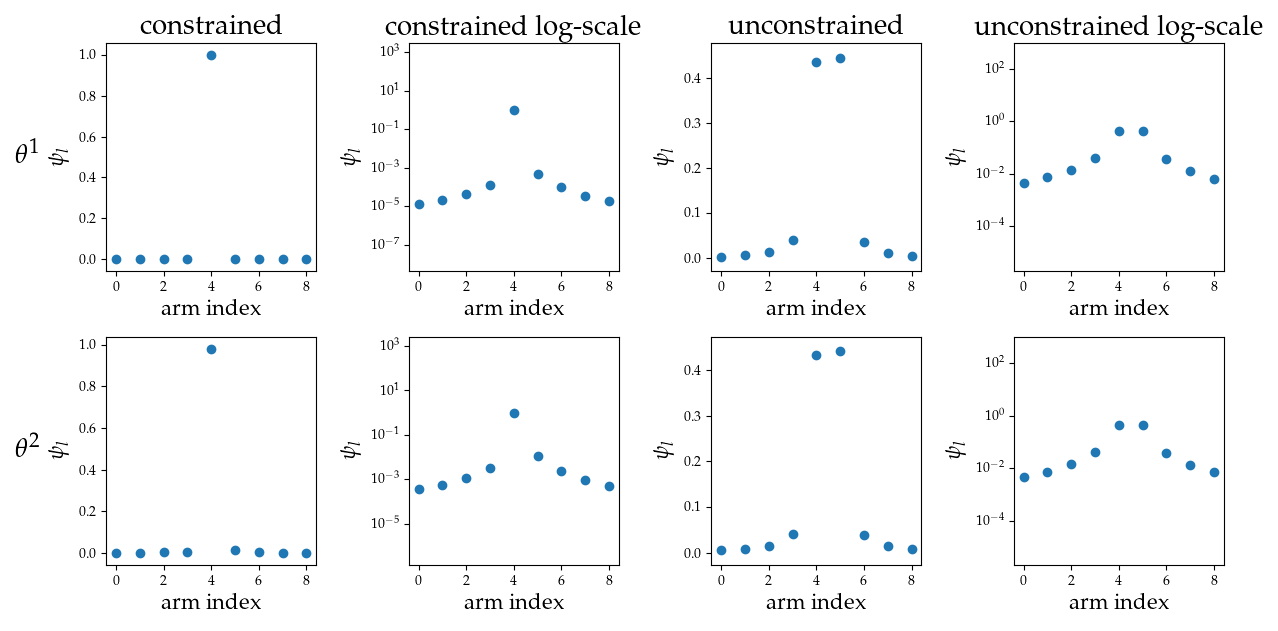
\includegraphics[width=\textwidth]{optimal_allocation.png}
  \caption{Unconstrained and constrained optimal allocation for $\theta_1$ and $\theta_2$, top-4}
  \label{fig:optimal_allocation}
\end{figure}

\section{A sufficient condition for
    optimality}\label{section:optimality_sufficient_condition}
This sufficient condition for convergence towards the optimal allocation is
centered around observing consequences of overallocation. Note that whenever an
allocation is different from the optimal allocation, this implies both over- and
underallocation. We focus on the statement for overallocation, yet an analogous
statement for underallocation should be possible.

In particular, the statement expresses that if an arm $l$ has been
over-allocated so far, indicated by a $\bar{\psi}_{n, l}$ larger than
$\psi^{\frac{1}{2}*}_l$, this over-allocation will be corrected. In this case,
correction means that its likelihood of being sampled in the next and round,
$\psi_{n, l}$ is very low. The intuition of the whole statement being that if
all overallocation is corrected for, then consequently all underallocation is
corrected for as well, by the fact that $\psi$ is a probability distribution.
\begin{proposition}\label{proposition:optimality_sufficient_condition}
  If
  \begin{align}
    \forall l \in [k], \delta > 0: \sum_{n \in \mathbb{N}} \psi_{n, l}
        \mathbb{I}[\bar{\psi}_{n, l} \geq \psi^*_l + \delta] < \infty
        \label{eq:sufficient_condition}
  \end{align}
  then $\bar{\psi}_{n} \rightarrow \psi^*$.
\end{proposition}

\section{Proofs}\label{section:optimal_proofs}
\begin{proof}[\Cref{lemma:set_relation_S*_i}]
  We first show the relationship between $\Theta_{S^*}^c$ and sets $\bar{\Theta}_i$ and then show the relationship between $\Theta_{S^*}^c$ and $\Theta_{m, j}$.
  \begin{align}
    \Theta_{S^*}^c &= \{\theta \in \Theta | \min_{j \in S^*} \theta_j > \max_{i \notin S^*} \theta_i \}^c \\
    &= \{\theta \in \Theta | \max_{i \notin S^*} \theta_i \geq \min_{j \in S^*} \theta_j\} \\
    &= \{\theta \in \Theta | \exists i \notin S^*: \theta_i \geq \min_{j \in S^*} \theta_j\} \\
    &= \{\theta \in \Theta | \exists i \notin S^*: \text{top-}m(\theta, S^* \cup \{i\}) \neq S^*\} \\
    &= \bigcup_{i \notin S^*} \{\theta \in \Theta | \text{top-}m(\theta, S^* \cup \{i\}) \neq S^*\} \\
    &= \bigcup_{i \notin S^*} \bar{\Theta}_i \\
    \Theta_{S^*} &= \{\theta \in \Theta | \min_{j \in S^*} \theta_j > \max_{j \in S^*} \theta_j\} \\
    &= \{\theta \in \Theta | \bigwedge_{j \in S^*} \theta_j > \max_{j \in S^*} \theta_j\} \\
    &= \bigcap_{j \in S^*} \{\theta \in \Theta | \theta_j > \max_{j \in S^*} \theta_j\} \\
    &= \bigcap_{j \in S^*} \{\theta \in \Theta | j \in \text{top-}m(\theta, [k])\} \\
    &= \bigcap_{j \in S^*} \Theta_{m, j} \\
    \Theta_{S^*}^c &= \Theta - \Theta_{S^*}\\
    \Theta_{S^*}^c &= \Theta - \bigcap_{j \in S^*} \Theta_{m, j}
  \end{align}
\end{proof}

\begin{proof}[\Cref{lemma:posterior_S*_i}]
  First, we prove the equality for $i \notin S^*$, followed by the equality for $j \in S^*$.

  The union from \Cref{lemma:set_relation_S*_i} has an additive effect with
  respect to the probability distribution $\Pi_n$. There are $k-m$ possible $i$s
  and each single one leads to a set, whose density is bounded by the maximal
  density of all such sets. This gives us:
  \begin{align}
    \max_{i \notin S^*} \Pi_n(\bar{\Theta}_i) \leq \Pi_n(\Theta_{S^*}^c) \leq (k-m) \max_{i \notin S^*} \Pi_n(\bar{\Theta}_i)
  \end{align}
  We use the definition of $\deq$ to compare lower bound and upper bound.
  \begin{align}
    \lim_{n \rightarrow \infty} \frac{1}{n} \log{\frac{\max_{i \notin S^*} \Pi_n(\bar{\Theta}_i)}{(k-m)\max_{i \notin S^*} \Pi_n(\bar{\Theta}_i)}}
    = \lim_{n \rightarrow \infty} \frac{1}{n} \log{\frac{1}{k-m}} \rightarrow 0
  \end{align}
  Thanks to the lower and upper bound being 'equal' in the $\deq$ sense, we can
  apply the Squeeze theorem\footnote{Also referred to as Sandwich teorem}. We
  obtain the desired result:
  \begin{align}
    \Pi_n(\Theta_{S^*}^c) \deq \max_{i \notin S^*} \Pi_n(\bar{\Theta}_i)
  \end{align}
  For $j \in S^*$, we follow a very similary path by first leveraging the set
  equality from \Cref{lemma:set_relation_S*_i}. Instead of a union, as was the
  case for $i \in S^*$, we are now confronted with an intersection. This implies
  a multiplicative effect on the distribution $\Pi_n$ instead of an additive
  one.
  \begin{align}
    &1 - \min_{j \in S^*} \Pi(\Theta_{m, j}) \leq \Pi(\Theta_{S^*}^c) \leq 1 - \min_{j \in S^*} (\Pi(\Theta_{m, j}))^m \\
  \end{align}
  Again, we will compare upper and lower bound in the $\deq$ sense.
  \begin{align}
    &\lim_{n \rightarrow \infty} \frac{1}{n} \log(\frac{\min_{j \in S^*} \Pi(\Theta_{m, j})}{\min_{j \in S^*} (\Pi(\Theta_{m, j}))^m}) = \lim_{n \rightarrow \infty} \frac{-(m - 1)}{n} \log(\min_{j \in S^*} \Pi(\Theta_{m, j}))
  \end{align}
  Observe that $1 \geq \min_{j \in S^*} \Pi(\Theta_{m, j}) \geq \alpha_{n, S^*} \rightarrow 1$. Hence the limit of the fraction goes to 0 and we have $\min_{j \in S^*} \Pi(\Theta_{m, j}) \deq \min_{j \in S^*} (\Pi(\Theta_{m, j}))^m$. Again, by the Squeeze theorem it follows that
  \begin{align}
    \Pi_n(\Theta_{S^*}^c) \deq 1 - \min_{j \in S^*} \Pi_n(\Theta_{m, j})
  \end{align}
\end{proof}

\begin{proof}[\Cref{lemma:kl_to_C}]
  \begin{align}
    \min_{\theta \in \bar{\Theta}_i} \sum_{j=1}^k \psi_j d(\theta^*_j||\theta_j)
      &= \min_{\theta \in \bar{\Theta}_i} \sum_{j\in S^*}
          \psi_{j}d(\theta^*_{j} || \theta_{j}) + \psi_{i}d(\theta_{i}^* ||
          \theta_{i}) + \sum_{j \notin S^* \cup \{i\}} \psi_j
          d(\theta^*_j||\theta_j) \\
      &= \min_{\theta \in \bar{\Theta}_i} \sum_{j\in S^*}
          \psi_{j}d(\theta^*_{j} || \theta_{j}) + \psi_{i}d(\theta_{i}^* ||
          \theta_{i}) \label{eq: l2_1}\\
      &= \min_{j\in S^*} \min_{\theta \in \bar{\Theta}_i}
          \psi_{j}d(\theta^*_{j} || \theta_{j}) + \psi_{i}d(\theta_{i}^* ||
          \theta_{i}) \label{eq: l2_2}\\
      &= \min_{j\in S^*} \min_{\theta \in \bar{\Theta}_i}
          \psi_{j}d(\theta^*_{j} || \theta_{j}) + \psi_{i}d(\theta_{i}^* ||
          \theta_{j}) \label{eq: l2_3}\\
      &= \min_{j\in S^*} \min_{x \in \mathbb{R}} \psi_{j}d(\theta^*_{j} || x) +
          \psi_{i}d(\theta_{i}^* ||x) \label{eq: l2_4}\\
      &= \min_{j \in S^*} C_{j, i}(\psi_j, \psi_i)
  \end{align}
  \eqref{eq: l2_1} follows from the fact that for any feasible $\theta$, we can
  define an alternative $\theta'$ s.t. $\theta'_i = \theta_i$, $\theta'_j =
  \theta_j$ for all $j \in S^*$ and $\theta'_{i_x} = \theta^*_{i_x}$ for all
  $i_x \notin S^* \cup \{i\}$. For such a $\theta'$, all terms involving $i_x
  \notin S^* \cup \{i\}$ are zero by the definition of the KL divergence while
  all others terms remain unchanged. Hence the minimum occurs with such a
  $\theta'$. Importantly, $\theta'$ remains feasible according to current
  definitions of $\bar{\Theta}_i$, i.e. $\theta' \in \bar{\Theta}_i$.

  \eqref{eq: l2_2} follows from a similar observation: only a single arm from
  $S^*$ needs to be inferior to arm $i$ under $\theta$. Recall that the terms of
  the individual arms do not influence each other. This implies that the
  minimization will gravitate towards setting all but one arm from $S^*$ in
  $\theta$ to the their true value - as the KL divergence is minimized for the
  true values. Hence the terms of all but one arm from $S^*$ will be cancelled
  out by the minimization. As $i$ remains superior to one arm in $S^*$, we have
  top-$m(\theta, S^* \cup \{i\}) \neq S^*$. Thereby such a $\theta$ is feasible
  according to $\bar{\Theta}_i$.

  \eqref{eq: l2_3} follows from monotonicity of the KL divergence, as displayed
  in \Cref{eq:kl_monotonicity}, combined with the possibility of $\theta_i =
  \theta_j$ tells us that the minimum will be reached in the case of equality.

  \eqref{eq: l2_4} follows from observing that our minimization over $\theta$
  has reduced to a minimization over $\theta_j$. The latter is a one-dimensional
  real.
  TODO: Why can we assume that distributions from the exponential family can be represented by a single scalar?
\end{proof}

\begin{proof}[\Cref{lemma:C_concave}]
  For the sake of clarity, let us define
  \begin{align}
    f(x, (\psi_j, \psi_i)) = \psi_j d(\theta_j^*||x) + \psi_i d(\theta_i^* || x)
  \end{align}
  Note that $C_{j, i}(\psi_j, \psi_i) = min_{x \in \mathbb{R}} f(x,(\psi_j, \psi_i))$. Clearly, $f$ is linear in $(\psi_j, \psi_i)$. According to Boyd and Vandenberghe (3.2.5) \cite{Boyd:2004:CO:993483}, the minimum over a family of linear functions is concave.
\end{proof}

\textbf{\Cref{lemma:C_unique_solution}}
Assume $A'(\theta)$ to be the mean observation under $\theta$. Given a $j \in S^*$, the solution to the minimization problem \eqref{eq:C} in $x$ is $\bar{\theta} \in \mathbb{R}$, satisfying:
\begin{align}
  A'(\bar{\theta}) = \frac{\psi_j A'(\theta_j^*) + \psi_i
      A'(\theta_i^*)}{\psi_j + \psi_i}
\end{align}
Therefore
\begin{align}
  C_{j, i}(\psi_j, \psi_i) = \psi_j d(\theta^*_j || \bar{\theta}) + \psi_i
      d(\theta^*_i || \bar{\theta})
\end{align}
\begin{proof}[\Cref{lemma:C_unique_solution}]
  By \Cref{eq:exponential_kl} we know that for the exponential family of probability distributions it holds that:
  \[d(\theta||\theta') = (\theta - \theta')A'(\theta) - A(\theta) + A(\theta')\]
  Applying this identity to the definition of $C_{j, i}$ \label{eq:C} for given $j$, $i$, $\psi_j$, $\psi_i$ gives us:
  \begin{align}
    &\psi_{j}d(\theta^*_{j} || x) + \psi_{i}d(\theta_{i}^* ||x) \\
    &=\psi_j ((\theta_j^* - x)A'(\theta_j^*) - A(\theta_j^*) + A(x)) + \psi_i((\theta_i^* - x)A'(\theta_i^*) - A(\theta_i^*) + A(x))\\
    &= -x(\psi_j A'(\theta_j^*) + \psi_i A'(\theta_i^*)) + A(x)(\psi_j + \psi_i) + c
  \end{align}
  Where $c$ is independent of $x$. As we seeks to minimize this quantity with respect to $x$, we differentiate it with respect to $x$ and set it to 0. This yields:
  \[A'(x) = \frac{\psi_j A'(\theta_j^*) + \psi_i A'(\theta_i^*)}{\psi_j + \psi_i}\]
\end{proof}

\begin{proof}[\Cref{lemma:C_strictly_increasing}]
  We will proceed to show for fixed $j \in S^*$ and $i \notin S^*$, $C_{j, i}$
  is increasing in its first argument $\psi_j$ as its second argument $\psi_i$
  follows by symmetry.

  Let us define $f(x, \psi_j, p) = \psi_j d(\theta_j^*||x) + p d(\theta_i^*||x)$
  which implies that $C_{j, i}(\psi_j, p) = \min_{x \in \mathbb{R}} f(x, \psi_j,
  p)$. We first show that $f$ is strictly increasing in $\psi_j$ and will use
  that to show that the initial claim.

  As the KL divergence is non-negative we have:
  \begin{align}
    f(x, \psi_j + \epsilon, p) &= \psi_j d(\theta_j^*||x) + \epsilon
        d(\theta_j^*||x) + p d(\theta_i^*||x) \\
      &> p d(\theta_i^*||x) + \psi_j d(\theta_j^*||x)\\
      &= f(x, \psi_j, p)
  \end{align}
  And therefore $f$ is strictly increasing in $\psi_j$.

  For a given $p$, we fix $\psi_{j1} < \psi_{j2}$ from $[0, 1]$ as well as their counterparts
  \begin{align}
    &x_1 = \argmin_{x \in \mathbb{R}} f(x, \psi_{j1}, p)
    &x_2 = \argmin_{x \in \mathbb{R}} f(x, \psi_{j2}, p)
  \end{align}
  Hence our goal is to show that $f(x_1, \psi_{j1}, p) < f(x_2, \psi_{j2}, p)$.
  By \Cref{lemma:C_unique_solution} both $x_1$ and $x_2$ are unique. Hence
  \begin{align}
    f(x_1, \psi_{j1}, \alpha) &< f(x_2, \psi_{j1}, \alpha) \\
    f(x_2, \psi_{j2}, \alpha) &< f(x_1, \psi_{j2}, \alpha)
  \end{align}
  As $f$ is strictly increasing in its second argument, it holds that $f(x_2,
  \psi_{j1}, \alpha) < f(x_2, \psi_{j2}, \alpha)$. Chaining those inequalities
  together we obtain:
  \begin{align}
    f(x_1, \psi_{j1}, \alpha) < f(x_2, \psi_{j1})  < f(x_2, \psi_{j2}) < f(x_1,
        \psi_{j2})
  \end{align}
\end{proof}

\begin{proof}[\Cref{proposition:characterization}]
  We prove in the following order: \eqref{itm:p7_i} \eqref{eq:condition_C} must
  hold for an optimal allocation, \eqref{itm:p7_ii} an optimal allocation is
  unique. After this, the remaining claim, namely that no other constrained
  allocation can be better, follows directly.
  \begin{enumerate}[(i)]
    \item \label{itm:p7_i} Suppose that $\psi^{\frac{1}{2}*}$ is optimal but does not satisfy \eqref{eq:condition_C}. Hence for some $i_1, i_2 \notin S^*, j_1, j_2 \in S^*$ with $(j_1, i_1) \neq (j_2, i_2)$:
    \[C_{j_1, i_1}(\psi^{\frac{1}{2}*}_{j_1}, \psi^{\frac{1}{2}*}_{i_1}) > C_{j_2, i_2}(\psi^{\frac{1}{2}*}_{j_2}, \psi^{\frac{1}{2}*}_{i_2})\]
    This implies:
    \[C_{j_1, i_1}(\psi^{\frac{1}{2}*}_{j_1}, \psi^{\frac{1}{2}*}_{i_1}) > \min_{i \notin S^*} \min_{j \in S^*}C_{j, i}(\psi^{\frac{1}{2}*}_j, \psi^{\frac{1}{2}*}_i) \]
    Consider the the measurement plan $\psi^\epsilon$ with
    \begin{itemize}
      \item $\psi^\epsilon_{i_1} = \psi^{\frac{1}{2}*}_{i_1} - \epsilon$
      \item $\psi^\epsilon_{j_1} = \psi^{\frac{1}{2}*}_{j_1} - \epsilon$
      \item $\forall l\notin \{i_1, j_1\}: \psi^\epsilon_l = \psi^{\frac{1}{2}*}_\gamma + \frac{2 \epsilon}{k-2}$
    \end{itemize}
    We can choose $\epsilon$ sufficiently small such that we preserve the inequality
    \begin{align}
      C_{j_1, i_1}(\psi^\epsilon_{j_1}, \psi^\epsilon_{i_1}) > C_{j_2, i_2}(\psi^\epsilon_{j_2}, \psi^\epsilon_{i_2})
    \end{align}
    while shifting enough measurement to all other arms such that
    \begin{align}
      \min_{i \notin S^*} \min_{j \in S^*} C_{j, i}(\psi^\epsilon_{j}, \psi^\epsilon_i) > \min_{i \notin S^*} \min_{j \in S^*} C_{j, i}(\psi^{\frac{1}{2}*}_j, \psi^{\frac{1}{2}*}_i)
    \end{align}
    Hence $\psi^\epsilon$ obtains more evidence on the worst possible pair than
    $\psi^{\frac{1}{2}*}$ and thereby achieves a better convergence rate
    \eqref{eq:constrained_optimal_gamma}. In other words, $\psi^{\frac{1}{2}*}$
    is not optimal, which is a contradiction.

    \item \label{itm:p7_ii} Suppose that there are optimal $\psi^1$, $\psi^2$,
    therefore both satisfying \eqref{eq:condition_C} with the exact same value
    $C^*$. It follows that there is at least one $l$ s.t. $\psi^1_{l} \neq
    \psi^2_{l}$. W.l.o.g. assume $l = i_x \notin S^*$ and $\psi^1_{i_x} >
    \psi^2_{i_x}$.

    We proceed by case distinction and show that each leads to a contradiction.
    \begin{itemize}
      \item Only one arm is disinct.

      For some $\epsilon > 0$ and any $j \in S^*$ have
      \begin{align}
        C_{j, i_x}(\psi^2_j, \psi^2_{i_x} + \epsilon) &= C_{j, i_x}(\psi^1_j, \psi^2_{i_x} + \epsilon) \\
        &= C_{j, i_x}(\psi^1_j, \psi^1_{i_x}) \\
        &= C^* \\
        &= C_{j, i_x}(\psi^2_j, \psi^2_{i_x})
      \end{align}
      Which is a contradiction as $\epsilon$ is positive $C_{j, i_x}$ strictly increasing by \Cref{lemma:C_strictly_increasing}.
      \item More that one arm is distinct, but they all belong to either $S^*$ or $S^{*c}$.

      As our distinct value so far comes from $S^{*c}$, let's also assume, w.l.o.g., $i_y \notin S^*$ with $i_y \neq i_x$.

      Note that independently of whether $\psi^1_{i_y} \geq \psi^2_{i_y}$ or $\psi^1_{i_y} < \psi^2_{i_y}$ holds, the previous argument can be applied for any $j \in S^*$.

      \item At least one arm is distinct in both $S^*$ and $S^{*c}$.

      Let's assume first that the distinctive optimal arm is $j_x \in S^*$.
      Observe that $\psi^1_{j_x} < \psi^2_{j_x}$ has to hold, otherwise both
      $i_x$ and $j_x$ were allocated more weight in $\psi^1$ than in $\psi^2$.
      By \Cref{lemma:C_strictly_increasing} we recall the increase of $C_{j_x,
      i_x}$ in both of its arguments. This implies greater evidence for $\psi^1$
      than for $\psi^2$, a contradiction to the assumption that both are
      optimal.

      Recall our constraint $\frac{1}{2} = \sum_{j \in S^*} \psi_l = \sum_{i \notin S^*} \psi_i$, which has to hold for both $\psi^1$ and $\psi^2$.
      Hence for $psi^1$'s over-allocation on $i_x$, there has to be an $i_y \notin S^*$ for which $\psi^1$ underallocates, compared to $psi^2$.
      Summarizing, we have:
      \begin{itemize}
        \item $\psi^1_{i_x} = \psi^2_{i_x} + \epsilon$
        \item $\psi^1_{j_x} = \psi^2_{j_x} - \epsilon'$
        \item $\psi^1_{i_y} = \psi^2_{i_y} - \epsilon''$
      \end{itemize}
      Combining this with the fact that all $C$ values from both $\psi^1$ and $\psi^2$ have to equal one another, we obtain:
      \begin{align}
        C_{j_x, i_y}(\psi^2_{j_x} - \epsilon', \psi^2_{i_y} - \epsilon'') &= C_{j_x, i_y}(\psi^1_{j_x}, \psi^1_{i_y}) \\
        &= C^* \\
        &= C_{j_x, i_y}(\psi^2_{j_x}, \psi^2_{i_y})
      \end{align}
      which, again, is a contradiction by the strictly increasing nature of $C_{j_x, i_y}$.
    \end{itemize}
  \end{enumerate}
\end{proof}

\begin{proof}[\Cref{proposition:optimality_sufficient_condition}]
  First, we prove that $\liminf_{n \rightarrow \infty} \bar{\psi}_{n, l} \leq \psi^*_l$ by contradiction.
  Assume otherwise. Then there are $n_0$ and $\delta$ such that for all $n > n_0:$ $\bar{\psi}_{n, l} \geq \psi^*_l + \delta$.
  \begin{align}
  \sum_{n \in \mathbb{N}} \psi_{n, i} &= \sum_{n \in [0, n_0]} \psi_{n, l} + \sum_{n \in [n_0 + 1, \infty]} \psi_{n, l} \\
  &= \sum_{n \in [0, n_0]} \psi_{n, l} +  \sum_{n \in [n_0 + 1, \infty]} \psi_{n, l}\mathbb{I}[\bar{\psi}_{n, l} \geq \psi^*_l + \delta]
  \end{align}
  The first term is finite as it consists of finitely many terms that are each finite themselves, in particular bounded from above by 1. The second term is finite by the assumption of the Lemma and the knowledge that $\psi$ is positive. Hence $\sum_{n \in \mathbb{N}} \psi_{n, l} < \infty$.
  \begin{align}
  \lim_{n \rightarrow \infty} \sum_{l \in [k]} \bar{\psi}_{n, l} = \lim_{n \rightarrow \infty} \sum_{l \in [k]} \frac{\sum_{n' \in [n]} \psi_{n', l}}{n} \rightarrow 0
  \end{align}
  However, we know by the definition of $\psi$ that for any $n$, $\sum_{n' \in [n]} \sum_{l \in [k]} \bar{\psi}_{n, l}  = n$, which is a contradiction.

  Second, we will prove that $\limsup_{n \rightarrow \infty} \bar{\psi}_{n, l}
  \leq \psi^*_l$ by contradiction. Assume otherwise. Combined with the previous
  point, this implies that for infinitely many $n$, $\bar{\psi}_{n, l}$ is above
  and for infinitely many it is below $\psi^*_l$. As $n$ belongs to a countable
  set, those points below and above have to alternate. This implies that our
  indicator function is 'triggered' infinitely many times. Observe that if
  $\psi_{n, l}$ is 0 once, it will never increase again as no posterior updates
  will be made. Hence every time the indicator function is triggered, $\psi_{n,
  l}$ has to be stricly positive; otherwise $l$ would never be sampled again and
  $\bar{\psi}_{n, l}$ monotonically decrease, even though it oscillates. As a
  consequence, we have an infinite amount of non-zero, positive values and hence
  \[\sum_{n \in \mathbb{N}} \psi_{n, l} \mathbb{I}[\bar{\psi}_{n, l} \geq
      \psi^*_l + \delta] = \infty\]
  which violates the assumption of the lemma and thereby is a contradiction.

  With the help of our initial assumption we know that for all $l$ it holds that
  $\limsup \bar{\psi}_{n, l} \rightarrow \psi^*_l$. This, combined with the fact
  that $\sum_{l \in [k]} \bar{\psi}_{n, l} = \sum_{l \in [k]} \psi^*_{l}$ allows
  us to conclude that $\bar{\psi}_{n} \rightarrow \psi^*$.
\end{proof}

\chapter{Top-2$m$ XOR Thompson Sampling}

In this chapter we will both present and analyze our suggested generalization of
Russo's Top-Two Thompson sampling: Top-2$m$ XOR Thompson sampling. The
underlying idea still revolves around repeatedly applying Thompson sampling
until two different candidates are at hand.

\Cref{section:algorithm} introduces the algorithm and provides some explanations
with regards to generalization decisions. It also introduces the constraint
$\psi_{S^*} = \frac{1}{2}$. Subsequently, \Cref{section:analysis} analyzes
properties of the algorithm. In particular it presents bounds on the measurement
plan, states general consequences of finite measurement and discusses
implications of underallocation and overallocation. We firmly believe that all
of those are very useful to show that this algorithm's measurement plan
converges to the optimal constrained measurement plan $\psi^{\frac{1}{2}*}$.
Proofs for those statements are provided in \Cref{section:txts_proofs}.
Additionally, we provide some empirical results in
\Cref{section:empirical_behavior}.

\section{Algorithm}\label{section:algorithm}
As a generalization of Russo's TTTS, the main difference lies in the fact that
candidates are sets. Hence Thompson sampling is repeated until set inequality is
reached. However, we can only ever sample individual arms, i.e. not sets. Hence
in this set scenario, we still need a mechanism to select a single arm from a
set. Therefore, when generalizing Russo's approach, the central and unavoidable
question arises: 'How to select a single arm from two unequal set candidates?'

According to a suggestion Russo gives in his outlook, we decided to tackle this
question by splitting it up into two steps.

First, given candidates $S_1$ and $S_2$ with $S_1 \neq S_2$, we compute the set
of elements which are contained in exactly one of both sets, i.e. the XOR of
both sets. Naturally, this restricted set is of cardinality at least 2.
Intuitively it points us towards arms which are 'uncertain'. Observe that arms
which are clearly suboptimal are very unlikely to appear in either $S_1$ or
$S_2$ through Thompson sampling. At the same time, arms that are clearly optimal
are very likely to appear in both $S_1$ and $S_2$ through Thompson sampling.
Hence arms that appear in only either of them are neither clearly optimal nor
clearly suboptimal.

As mentioned before, the XOR of $S_1$ and $S_2$ will always contain at least two
elements. Hence we need to define an approach on how to select from the XOR.
According to both Russo's suggestion as well as Occam's razor, we opted for
uniform selection.

We believe that the applying a XOR to both candidates is essential for the
correctness of the algorithm, whereas the uniform sampling from the XOR of both
candidates could easily be substituted by other distributions. We would expect
such a change to preserve correctness, as long as every arm of the XOR is
sampled with strictly positive probability. Yet, it would likely alter the
hyperparamter $\beta = \psi_{S^*}$.

We present the approach to sample an arm in step $n + 1$ in \Cref{alg:TXTS}.
This approach can be repeated either for a fixed amount of samples or until a
specific confidence level is reached. Note that the confidence level can be
approximated in every step. The confidence level is equal to $\Pi_n(\Theta_S)$
where $S = \argmax_{S'} \Pi_n(\Theta_{S'})$. Concretely, this quantity can be
estimated by drawing samples from $\Pi_n$ and identifying for which set $S$ the
fraction $\frac{\text{\# samples in which $S$ is optimal}}{\#samples}$ is
largest. The fraction of this $S$ approximates the confidence level.
\begin{algorithm}[H]
  \caption{Given a posterior $\Pi_n$ in step $n+1$}
  \label{alg:TXTS}
  \begin{algorithmic}
    \State $\hat{\theta} \sim \Pi_n$
    \State $S_1 =$ top-$m(\hat{\theta})$
    \Repeat
      \State $\hat{\theta} \sim \Pi_n$
      \State $S_2 = $ top-$m(\hat{\theta})$
    \Until{$S_1 \neq S_2$}
    \State $I_{n+1} \sim \mathcal{U}(S_1 \oplus S_2)$
    \State Play $I_{n+1}$, observe reward and update posterior
  \end{algorithmic}
\end{algorithm}
We expect this algorithm to induce a measurement plan $\psi$ such that
$\psi_{S^*} = \frac{1}{2}$. This expectation gives rise to the constrained
optimization from the previous chapter. Note that this constraint is a
consequence of the design decision of which operation to apply to candidates
$S_1$ and $S_2$.

\section{Analysis}\label{section:analysis}
Starting off by a statement about the implications of finite measurement, we
later establish bounds and equalities on the measurement plan $\psi$ of the
algorithm.

The following lemma formalizes two three seemingly intuitive statements. First,
it shows that for each arm that is sampled infinitely many times, the estimated
mean will converge to its true mean. Second, it demonstrates that if every arm
is sampled infinitely often, the posterior will put all of its mass on
parameters with $S^*$ as top-$m$ arms. Third, it argues that as long as some
arms have only been granted finite measurement, they can't be ruled out from
being optimal.
\begin{lemma}\label{lemma:finite_measurement}
  $\mathcal{I} = \{l: \sum_{n=1}^\infty \psi_{n, l} < \infty\}$
  \begin{itemize}
    \item $\forall l \notin \mathcal{I}, \forall \epsilon: \Pi_n(\{\theta:
        \theta_l \in (\theta^*_l - \epsilon, \theta^*_l + \epsilon)\})
        \rightarrow 1$
    \item $\mathcal{I} = \emptyset \Rightarrow
    \alpha_{n, S} \rightarrow \begin{cases}
      1 & \text{if } S = S^*\\
      0 & \text{if } S \neq S^*
    \end{cases}$
    \item $\forall S \subset \mathcal{I}: \liminf_{n \rightarrow \infty}
        \alpha_{n, S} > 0$
  \end{itemize}
\end{lemma}
Going on to expressing the measurement plan, we observe that a closed-form
equality is not easy to obtain. In comparison to Russo's case, it is much harder
to construct a closed-form probability of arm $l$ being sampled in a given step
as there are many more different scenarios. Vaguely speaking, the XORs can be of
very different kinds.

In this spirit, we offer both lower and upper bounds on the measurement plan of
a single arm. The overall idea is to case-distinguish if $l$ lies set $S_1$ or
$S_2$. Facing the probability of $l$ being selected given its belonging to the
XOR, we leverage the knowledge of the uniform draw. Hence we have $\Pr[I_n = l|l
\in S_1 \oplus S_2] = \frac{1}{|S_1 \oplus S_2|}$. The cardinality of the XOR
can be trivially bounded from below by 2 or from above by 2$m$. Note that these
inequalities are tight with respect to $n$ as $m$ can be seen as a constant.
\begin{proposition}\label{proposition:measurement_plan_arm}
  \begin{align}
    \psi_{n, l} &\leq \frac{1}{2}(\sum_{S: l \in S} \frac{\alpha_{n, S}}{1 -
        \alpha_{n, S}} (1 - \alpha_{n, l}) +  \sum_{S': l \notin S'}
        \frac{\alpha_{n, S'}}{1 - \alpha_{n, S'}} \alpha_{n, l}) \\
    \psi_{n, l} &\geq \frac{1}{2m}(\sum_{S: l \in S} \frac{\alpha_{n, S}}{1 -
        \alpha_{n, S}} (1 - \alpha_{n, l}) +  \sum_{S': l \notin S'}
        \frac{\alpha_{n, S'}}{1 - \alpha_{n, S'}} \alpha_{n, l})
  \end{align}
\end{proposition}
Having established bounds on the measurement plan for individual arms, we
proceed to establish two equalities on the measurement plan for sets. In this
case we neither propose a closed-form solution nor a bound. Rather, we veil some
of the uncertainty with a probability term, which turns out to be sufficiently
expressive for some of the later applications.
\begin{proposition}\label{proposition:measurement_pan_set}
  \begin{align}
    \psi_{n, S} &= \frac{1}{2} \alpha_{n, S} +  \Pr[I_n \in S | S_1 \neq S] (1 - \alpha_{n, S}) \\
    \psi_{n, S} &= \frac{\alpha_{n, S}}{2} +  \frac{\alpha_{n, S}}{2} \sum_{S'\neq S} \frac{\alpha_{n, S'}}{1 - \alpha_{n, S'}} + \Pr[S_1, S_2 \neq S \wedge I_n \in S]
  \end{align}
\end{proposition}
This form of $\psi_{n, S}$ allows us to deduct that the algorithm collects infinite measurement on every arm given infinite samples.
\begin{lemma}\label{lemma:infinite_measurement}
  \begin{align}
    \sum_{n \in \mathbb{N}} \psi_{n, S} \rightarrow \infty
  \end{align}
\end{lemma}
Recalling \Cref{lemma:finite_measurement}, this is particularly interesting as it signals that for $n \rightarrow \infty$ we have that $\mathcal{I} = \emptyset$. Therefore $\alpha_{n, S^*} \rightarrow 1$ holds true, too.
Having established $\psi_{n, S}$ as function of $\alpha_{n, S}$, we continue by analyzing the effect of $\alpha_{n, S} \rightarrow 1$ on $\psi_{n, S}$, for general $S$, followed by the application on $S^*$.
\begin{lemma}\label{lemma:psi_convergence}
  \begin{align}
    \alpha_{n, S} \rightarrow 1 \Rightarrow \psi_{n, S} \rightarrow \frac{1}{2}
  \end{align}
\end{lemma}
This result confirms our hunch about the constraint induced of the algorithm:
once it becomes 'sure' of the optimality of a set $S$, it will sample arms from
it with probability $\frac{1}{2}$. As we have previously argued, we have that
$\alpha_{n, S^*} \rightarrow 1$ and therefore $\psi_{n, S^*} \rightarrow
\frac{1}{2}$.

Moreover, once we know that $\alpha_{n, S^*} \rightarrow 1$, we can simplify the
bound from \Cref{proposition:measurement_plan_arm}.
\begin{lemma}\label{lemma:measurement_plan_bound_max}
  If $\alpha_{n, S^*} \rightarrow 1$, then for all $i \notin S^*$ and for all
  $j \in S^*$:
  \begin{align}
    \psi_{n, i} &\leq \frac{\alpha_{n, i}}{\max_{S' \neq S^*} \alpha_{n, S'}} \\
    \psi_{n, j} &\leq \frac{1 - \alpha_{n, j}}{\max_{S' \neq S^*} \alpha_{n,
        S'}}
  \end{align}
\end{lemma}

\section{Empirical behavior}\label{section:empirical_behavior}
%What true distributions are assumed?
%What prior and posterior distributions are assumed?
%How is C computed?
%How is alpha computed, as it is defined via a huge integral?
%How is psi computed, as there is no closed form?

TODO: Talk about updates of priors.

For the following empirical results we assumed the rewards of arms to follow
Bernoulli distributions with means $\theta^* = [.1, .2, .3, .4, .5, .6, .7, .8,
.9]$. We defined priors/posteriors to be Beta distributed with initial
parameters $\alpha = \beta = 1$, mimicking a uniform prior on the set of arms.

The posterior mass put on certain events, in particular the confidence, were
computed as described in \Cref{section:algorithm}. \Cref{fig:confidences}
indicates the confidence for a given number of steps of our method compared to
the the uniform allocation and Thompson sampling.
\begin{figure}[h]
  \centering
  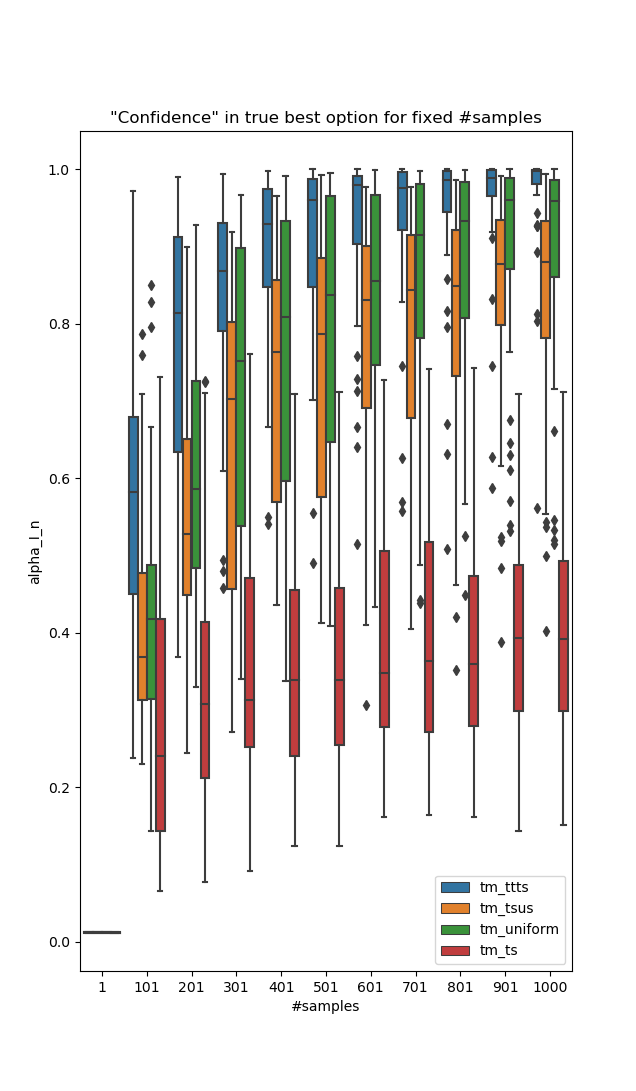
\includegraphics[width=.5\textwidth]{190723-confidences.png}
  \caption{Unconstrained and constrained optimal allocation for $\theta_1$ and $\theta_2$, top-4}
  \label{fig:confidences}
\end{figure}
As we don't have a closed form for the average measurement plan
$\bar{psi}_{n,l}$ at our disposal, we approximate it with the empirical sampling
frequencies. \Cref{fig:measurement_plan} indicates said empirical sampling
frequencies. Note that $\bar{psi}_{S^*}$ can nicely be read to equal
$\frac{1}{2}$.
\begin{figure}[h]
  \centering
  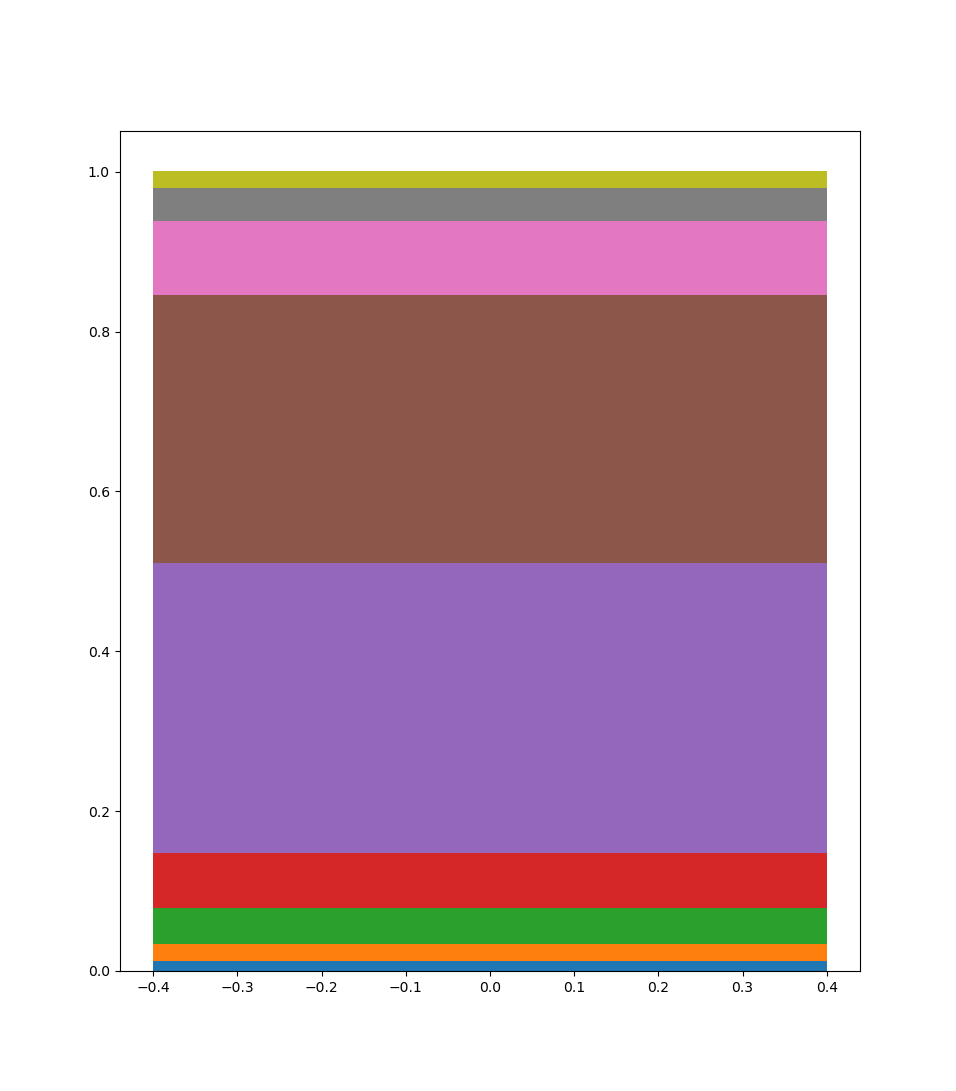
\includegraphics[width=\textwidth]{190723-selections_2.png}
  \caption{Unconstrained and constrained optimal allocation for $\theta_1$ and
  $\theta_2$, top-4}
  \label{fig:measurement_plan}
\end{figure}
As we know from \Cref{section:optimal_statements}, the optimal allocation
gathers equal evidence for all pairs from $S^* \times S^{*c}$. We used the
empirical sampling frequencies to approximate those coefficients. A qualitative
comparison of the individual coefficients can be found in
\Cref{fig:algorithm_coefficients}. The individual $C_{j, i}$ were computed just
as described in \Cref{section:concrete_optimal_allocation}.
\begin{figure}[h]
  \centering
  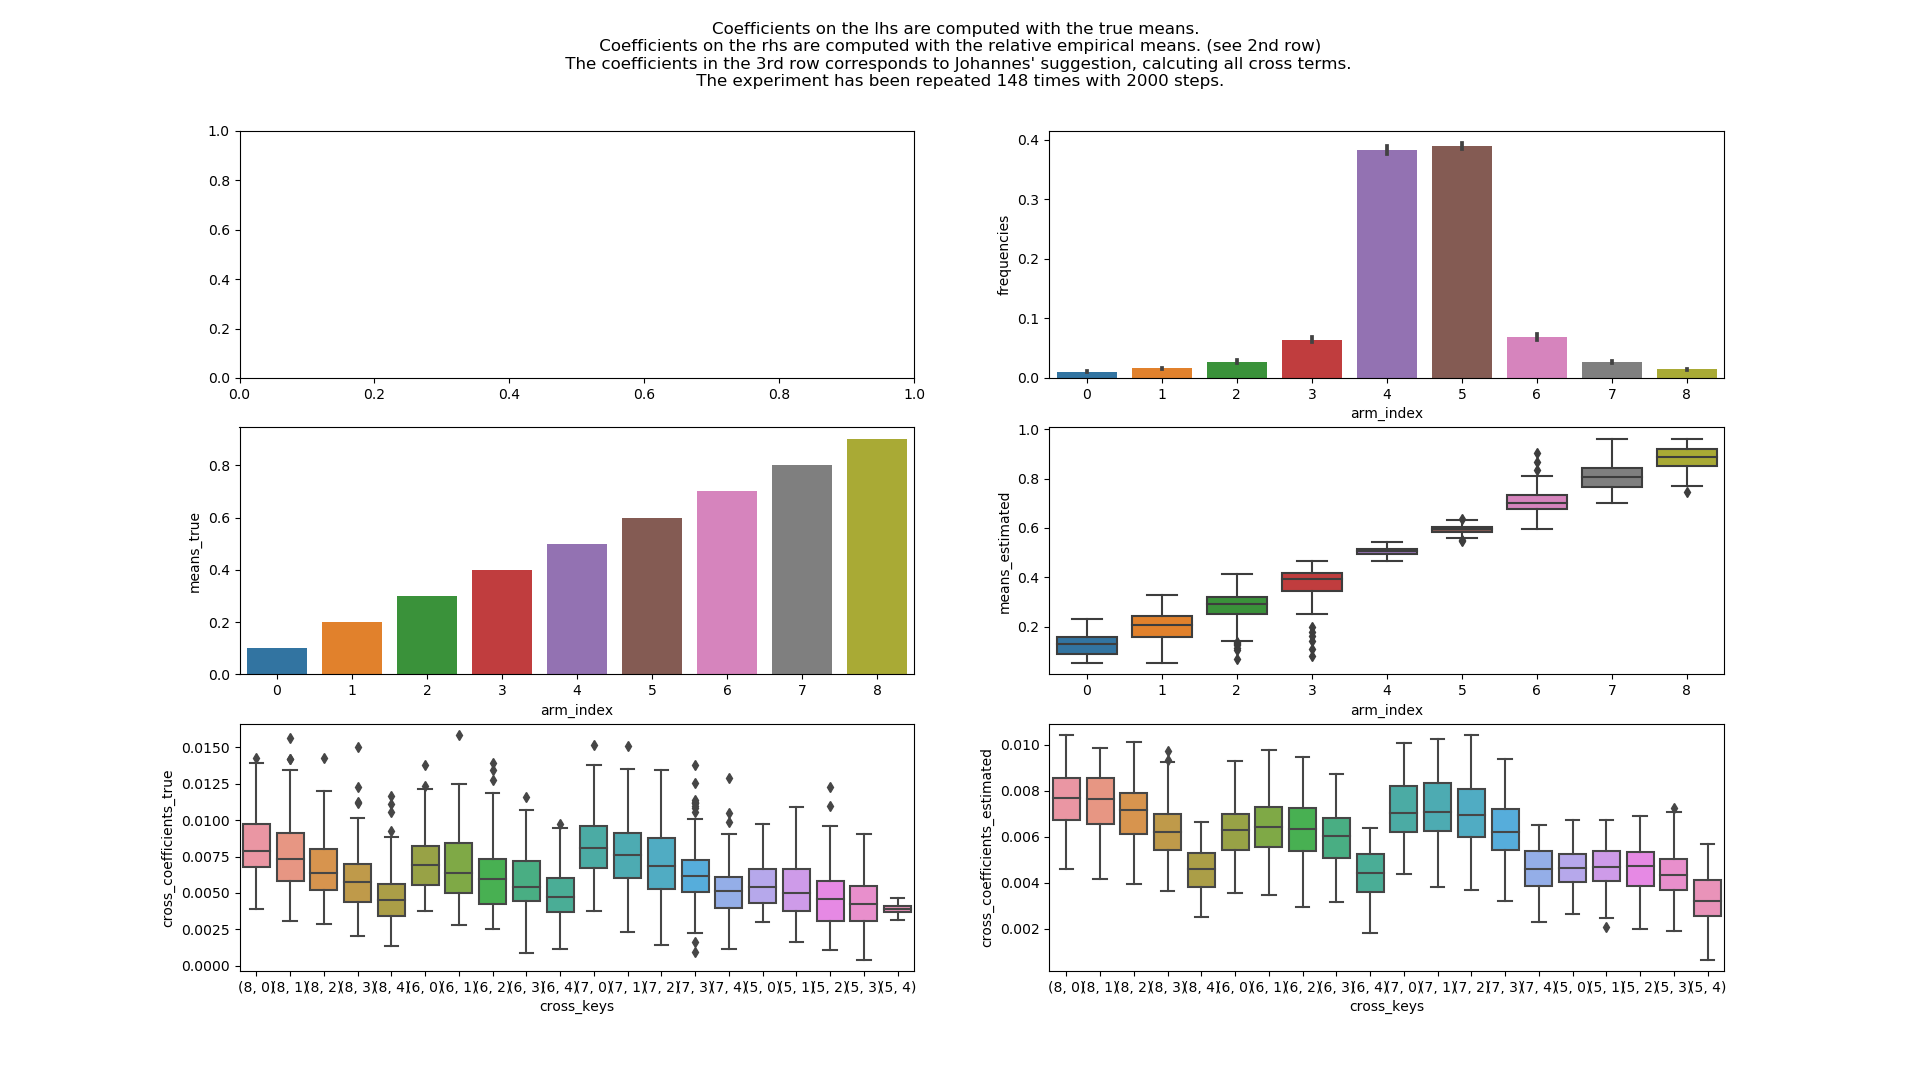
\includegraphics[width=\textwidth]{190909-coefficients_2000.png}
  \caption{Unconstrained and constrained optimal allocation for $\theta_1$ and
  $\theta_2$, top-4}
  \label{fig:algorithm_coefficients}
\end{figure}

\section{Further results}

\begin{lemma}\label{lemma:limsup_undersampling}
  Given $\sum_n(\frac{1}{2} - \psi_{l, n}) \mathbb{I}[\psi_{l, n} \leq \psi_l^*
  - \delta] < \infty$ we have that
  \[\limsup \bar{\psi}_{l, n} \geq \psi_j^* \text{ and } \liminf \bar{\psi}_{l,
  n} \geq \psi_j^*\]
\end{lemma}

\begin{lemma}\label{lemma:psi_undersampled}
  \begin{align}
    \psi_{n, \hat{j}} \geq \frac{1}{2} - m\exp(-n \delta)
  \end{align}
\end{lemma}

\section{Proofs}\label{section:txts_proofs}
\begin{proof}[\Cref{lemma:finite_measurement}]

  \begin{itemize}
  \item Note that this statement is equal for top-1 and top-$m$. Hence we can
  employ Russo's Proposition 4 telling us that if$\sum_{n \in \mathbb{N}}
  \psi_{n, l} \rightarrow \infty$, it follows that
  \begin{align}
    \Pi_n(\{\theta: \theta_l \in (\theta^*_l - \epsilon, \theta^*_l +
        \epsilon)\}) \rightarrow 1 \label{eq:concentration}
  \end{align}
  Hence \eqref{eq:concentration} holds for any $l \notin \mathcal{I}$. \item If
  $\mathcal{I} = \emptyset$, every arm is sampled infinitely often when the
  number of samples goes to infinity. This means that \eqref{eq:concentration}
  holds for every arm. In other words, our estimate of each arm is arbitrarily
  concentrated around its true value, i.e. $\Pi_n(\{\theta^*\}) \rightarrow 1$.
  Recalling our definitions of $S^*$, $\Theta_S$ and $\alpha_{n, S}$, we see
  that
  \[ \alpha_{n, S^*} = \Pi_n(\Theta_{S^*}) \geq \Pi_n(\{\theta^*\}) \rightarrow
      1\]
  As $\alpha_{n, S}$ is bounded by $[0, 1]$, we obtain the desired statement.
  \item As a syntactic alteration on $\theta_S$, let's define $\theta_{S,
  \epsilon} = \{\theta \in \Theta | \min_{j \in S} \theta_j \geq \max_{i \notin
  S} \theta_i + \epsilon\}$. Also, let us define $\rho^* = \max_{S \not\subseteq
  \mathcal{I}} \min_{i \in S} \theta^*_i$. Intuitively, $\rho^*$ represents a
  metric on the best set of arms under the true values, of which every arm is
  sampled infinitely often under infinite samples. Choose $\epsilon$ such that
  $\rho^* + 2\epsilon < \bar{\theta}$. For $S \subset \mathcal{I}$, we have:
  \begin{align}
    \theta_{S, \epsilon} &= \{\theta|(\min_{j \in S} \theta_j \geq \max_{i \in
        \mathcal{I} \setminus S} \theta_i + \epsilon) \wedge (\min_{j \in S}
        \theta_j \geq\ \max_{i \notin \mathcal{I}, S} \theta_i + \epsilon)\} \\
      &= \{\theta | (\forall i \in \mathcal{I} \setminus S: \min_{j \in S} \geq
          \theta_i + \epsilon) \wedge (\min_{j \in S} \theta_j \geq\ \max_{i
          \notin \mathcal{I}, S} \theta_i + \epsilon)\} \\
      & \supseteq \{\theta |(\min_{j \in S} \theta_j \geq \rho^* + 2 \epsilon)
          \wedge (\forall i \in \mathcal{I} \setminus S: \rho^* > \theta_i)
          \wedge (\min_{j \in S} \theta_j \geq\ \max_{i \notin \mathcal{I}, S}
          \theta_i + \epsilon)\} \\
      & \supseteq \{\theta |(\min_{j \in S} \theta_j \geq \rho^* + 2 \epsilon)
          \wedge (\forall i \in \mathcal{I} \setminus S: \rho^* > \theta_i)
          \wedge (\rho^* + \epsilon \geq \max_{i \notin \mathcal{I}, S}
          \theta_i)\} \\
      &= \underbrace{\{\theta |(\min_{j \in S} \theta_j \geq \rho^* + 2
          \epsilon) \wedge (\forall i \in \mathcal{I} \setminus S: \rho^* >
          \theta_i) \}}_\text{A} \setminus \underbrace{\{\theta| \max_{i \notin
          \mathcal{I}, S} \theta_i > \rho^* + \epsilon\}}_\text{B}
  \end{align}
  Where the last step follows from the fact that $\{x|p(x) \wedge q(x)\} =
  \{x|p(x)\} \setminus \{x|\neg q(x)\}$. By \eqref{eq:concentration}, we know
  that $\Pi_n(B) \rightarrow 0$. The second part of Russo's Proposition 4 tells
  us that over any open interval $(\theta_l', \theta_l'')$, we have $\inf_{n \in
  \mathbb{N}} \Pi_n(\{\theta| \theta_l \in (\theta_l', \theta_l'')\ \forall l
  \in \mathcal{I}\}) > 0$. By defining $(\theta_l', \theta_l'')$ to be $(\rho +
  2 \epsilon, \bar{\theta})$ for all arms from $S \subset \mathcal{I}$ and
  $(\underline{\theta}, \rho^* + \epsilon)$ for all arms in $\mathcal{I}
  \setminus S$, we get $\inf_{n \in \mathbb{N}} \Pi_n(A) > 0$. Together, this
  gives us
  \begin{align}
    \inf_{n \in \mathbb{N}} \alpha_{n, S} &= \inf_{n \in \mathbb{N}}
        \Pi_n(\theta_{S, \epsilon}) \geq \inf_{n \in \mathbb{N}}(\Pi_n(A) -
        \Pi_n(B)) > 0 \\
    \liminf_{n \in \mathbb{N}} \alpha_{n, S} &\geq \inf_{n \in \mathbb{N}}
        \alpha_{n, S} > 0
  \end{align}
  \end{itemize}
\end{proof}

\begin{remark}[Kevin 19/09/05]
  Why did we need $2\epsilon$ instead of $\epsilon$?
\end{remark}

\begin{proof}[\Cref{proposition:measurement_plan_arm}]
  It will prove itself useful to first investigate the probability of a given
  arm $l$ belonging to either $S_1$ or $S_2$, yet not both.
  \begin{align}
    &\Pr[l \in S_1 \wedge l \notin S_2] + \Pr[l \notin S_1 \wedge l \in S_2]  \\
    =& \sum_{S: l \in S} \Pr[S_1 = S] \sum_{S': l \notin S'} \Pr[S_2 = S' | S_1
        = S] + \\
    & \sum_{S': l \notin S'} \Pr[S_1 = S'] \sum_{S: l \in S} \Pr[S_2 = S | S_1
        = S'] \\
    =& \sum_{S: l \in S} \alpha_{n, S} \sum_{S': l \notin S'} \frac{\alpha_{n,
        S'}}{1 - \alpha_{n, S}} + \sum_{S': l \notin S'} \alpha_{n, S'}
        \sum_{S: l \in S} \frac{\alpha_{n, S}}{1 - \alpha_{n, S'}}\\
    =& \sum_{S: l \in S} \frac{\alpha_{n, S}}{1 - \alpha_{n, S}} \sum_{S': l
        \notin S'} \alpha_{n, S'} + \sum_{S': l \notin S'} \frac{\alpha_{n,
        S'}}{1 - \alpha_{n, S'}} \sum_{S: l \in S} \alpha_{n, S}\\
    =& \sum_{S: l \in S} \frac{\alpha_{n, S}}{1 - \alpha_{n, S}} (1 -
        \alpha_{n, l}) +  \sum_{S': l \notin S'} \frac{\alpha_{n, S'}}{1 -
        \alpha_{n, S'}} \alpha_{n, l}
  \end{align}
  This identity can now be leveraged for both lower and upper bound. But first,
  let's express the the measurement plan exactly.
  \begin{align}
    \psi_{n, l} =& \Pr[l \in S_1 \wedge l \notin S_2 \wedge I_n = l] + \Pr[l
        \notin S_1 \wedge l \in S_2 \wedge I_n = l] \\
    =& \Pr[I_n = l | l \in S_1 \wedge l \notin S_2] \Pr[l \in S_1 \wedge l
        \notin S_2] + \\
    & \Pr[I_n = l | l \notin S_1 \wedge l \in S_2] \Pr[l \notin S_1 \wedge l
        \in S_2]
  \end{align}
  Observe that both terms $\Pr[I_n = l | l \in S_1 \wedge l \notin S_2]$ and
  $\Pr[I_n = l | l \notin S_1 \wedge l \in S_2]$ correspond to a very similar
  situation: we know that $l$ is part of the XOR, but we don't know how exactly
  the rest of the XOR looks like. To those quantities we can apply the
  aforementioned naïve bounds of $\frac{1}{2}$ and $\frac{1}{2m}$.
  \begin{align}
    \psi_{n, l} \leq& \frac{1}{2} (\Pr[l \in S_1 \wedge l \notin S_2] + \Pr[l
        \notin S_1 \wedge l \in S_2]) \\
        =& \frac{1}{2}(\sum_{S: l \in S} \frac{\alpha_{n, S}}{1 - \alpha_{n,
            S}} (1 - \alpha_{n, l}) +  \sum_{S': l \notin S'} \frac{\alpha_{n,
            S'}}{1 - \alpha_{n, S'}} \alpha_{n, l}) \\
    \psi_{n, l} \geq& \frac{1}{2m} (\Pr[l \in S_1 \wedge l \notin S_2] + \Pr[l
        \notin S_1 \wedge l \in S_2]) \\
      \geq& \frac{1}{2m}(\sum_{S: l \in S} \frac{\alpha_{n, S}}{1 - \alpha_{n,
          S}} (1 - \alpha_{n, l}) +  \sum_{S': l \notin S'} \frac{\alpha_{n,
          S'}}{1 - \alpha_{n, S'}} \alpha_{n, l})
  \end{align}
\end{proof}

\begin{proof}[\Cref{proposition:measurement_pan_set}]
  In order to show the first equality, we rely on the idea that we only check
  if the first sampled set $S_1$ is equal to $S$.
  \begin{align}
    \psi_{n, S} &= \Pr[I_n \in S] \\
      &= \Pr[S_1 = S \wedge I_n \in S_1] + \Pr[S_1 \neq S \wedge I_n \in S] \\
      &= \Pr[I_n \in S_1 | S_1 = S] \Pr[S_1 = S] + \Pr[I_n \in S| S_1 \neq
          S]\Pr[S_1 \neq S] \\
      &= \Pr[I_n \in S_1] \Pr[S_1 = S] + \Pr[I_n \in S| S_1 \neq S](1 - \Pr[S_1
          = S]) \\
      &= \frac{1}{2} \alpha_{n, S} +  \Pr[I_n \in S | S_1 \neq S] (1 -
          \alpha_{n, S})
  \end{align}
  In order to show the second equality, we go a step further by checking if
  either of both sets equals $S$. For that purpose we first look into the
  probability that $S$ is sampled as a second set and that $I_n$ stems from $S$.
  \begin{align}
    & \sum_{S'\neq S}\Pr[S_1 = S' \wedge S_2 = S \wedge I_n \in S_2] \\
    &= \sum_{S'\neq S} \Pr[S_1 = S'] \Pr[S_2 = S | S_1 = S'] \Pr[I_n \in S_2 |
        S_1 = S' \wedge S_2 = S] \\
    &= \sum_{S'\neq S} \alpha_{n, S'} \frac{\alpha_{n, S}}{1 - \alpha_{n, S'}}
        \frac{1}{2} = \frac{\alpha_{n, S}}{2} \sum_{S'\neq S} \frac{\alpha_{n,
        S'}}{1 - \alpha_{n, S'}}
  \end{align}
  \begin{align}
    \psi_{n, S} =& \Pr[I_n \in S] \\
      =& \Pr[S_1 = S \wedge I_n \in S_1] + \Pr[S_2 = S \wedge I_n \in S_2] +
          \Pr[S_1, S_2 \neq S \wedge I_n \in S]\\
      =& \frac{\alpha_{n, S}}{2} + \sum_{S'\neq S}\Pr[S_1 = S' \wedge S_2 = S
          \wedge I_n \in S_2] +  \Pr[S_1, S_2 \neq S \wedge I_n \in S] \\
      &= \frac{\alpha_{n, S}}{2} +  \frac{\alpha_{n, S}}{2} \sum_{S'\neq S}
          \frac{\alpha_{n, S'}}{1 - \alpha_{n, S'}} + \Pr[S_1, S_2 \neq S
          \wedge I_n \in S]
    \end{align}
\end{proof}

\begin{proof}[\Cref{lemma:infinite_measurement}]
  \Cref{proposition:measurement_pan_set} tells us that $\psi_{n, S} > \gamma
  \alpha_{n, S}$ for some constant $j > 0$. Thanks to this we have $\sum_{n \in
  \mathbb{N}} \psi_{n, S} > \frac{1}{2} \sum_{n \in \mathbb{N}} \alpha_{n, S}$.
  For the sake of contradiction, assume that $\exists S'$ with $\sum_{n \in
  \mathbb{N}} \psi_{n, S'} < \infty$. According to
  \Cref{lemma:finite_measurement}'s definition, we have $S \subset \mathcal{I}$.
  Hence we can apply its third clause and get $\liminf_{n \rightarrow \infty}
  \alpha_{n, S'} > 0$. Using our initial bound we observe that we have an
  infinite sum of terms which have a $\liminf$ greater than 0. Hence $\sum_{n
  \in \mathbb{N}} \psi_{n, S}$ tends to infinity with growing $n$ and the
  assumption is contradicted.
\end{proof}

\begin{proof}[\Cref{lemma:psi_convergence}]
  In \Cref{proposition:measurement_pan_set}'s first form,  $\Pr[I_n \in S | S_1
  \neq S]$ is naturally bounded by 1. The desired statement follows immediately.
\end{proof}

\begin{proof}[\Cref{lemma:measurement_plan_bound_max}]
  \Cref{proposition:measurement_plan_arm} tells us that
  \[\psi_{n, l} \leq \frac{1}{2}(\sum_{S: l \in S} \frac{\alpha_{n, S}}{1 -
      \alpha_{n, S}} (1 - \alpha_{n, l}) +  \sum_{S': l \notin S'}
      \frac{\alpha_{n, S'}}{1 - \alpha_{n, S'}} \alpha_{n, l})\]
  Knowing that $\alpha_{n, S^*} \rightarrow 1$, we can bound $\psi_{n, i}$ in
  the following way:
  \begin{align}
    \psi_{n, i} \leq& \frac{1}{2}((1 - \alpha_{n, i}) \frac{\sum_{S: i \in S}
        \alpha_{n, S}}{1 - \alpha_{n, S^*}} + \alpha_{n, i} \frac{\sum_{S': i
        \notin S'} \alpha_{n, S'}}{1 - \alpha_{n, S^*}}) \\
      =& \frac{1}{2}((1 - \alpha_{n, i}) \frac{\alpha_{n, i}}{1 - \alpha_{n,
          S^*}} + \alpha_{n, i} \frac{1 - \alpha_{n, i}}{1 - \alpha_{n, S^*}})\\
      \leq& \frac{1}{2} \frac{2 \alpha_{n, i} (1 - \alpha_{n, i})}{\max_{S'
          \neq S^*} \alpha_{n, S'}} \\
      \leq& \frac{\alpha_{n, i}}{\max_{S' \neq S^*} \alpha_{n, S'}}
  \end{align}
  for $i \notin S^*$ as well as
  \begin{align}
    \psi_{n, j} \leq& \frac{1 - \alpha_{n, j}}{\max_{S' \neq S^*} \alpha_{n,
        S'}}
  \end{align}
  for $j \in S^*$.
\end{proof}

\begin{proof}[\Cref{lemma:limsup_undersampling}]
    We first show the first statement and then use it for the second. For the
    sake of contradiction, we assume that $\limsup \bar{\psi}_{l, n} <
    \psi_j^*$. This implies that there is a $n_0$ from which onward $\psi_{l,
    n} < \psi_l^*$.
    \begin{align}
      \sum_n (\frac{1}{2} - \psi_{l, n}) &= \sum_{n=1}^{n_0} (\frac{1}{2} -
          \psi_{l, n}) + \sum_{n > n_0} (\frac{1}{2} - \psi_{l, n}) \\
        &= \sum_{n=1}^{n_0} (\frac{1}{2} - \psi_j) + \sum_{n > n_0}
            (\frac{1}{2} - \psi_{l, n})\mathbb{I}[\psi_{l, n} \leq \psi_l^* -
            \delta] \\
        &= C
    \end{align}
    Where the last line follows from the assumption and the fact that the first
    sum is a finite amount of individually finite quantities. Hence we can
    write:
    \begin{align}
      \sum_n \psi_{l, n} &= -C + \sum_n \frac{1}{2} \\
      \bar{\psi}_{l, n} &= \frac{-C}{n} + \frac{1}{2}\sum_n\frac{1}{n} \\
        &= \frac{-C}{n} + \frac{1}{2} H_n
    \end{align}
    We know that $H_n$ is asymptotically equivalent to $\log(n)$. Hence we get
    that $\bar{\psi}_{l, n} \rightarrow \infty$, which is a contradiction.
    Therefore we have $\limsup \bar{\psi}_{l, n} \geq \psi_j^*$.

    The argument from Lemma 9 can be repeated to show the second statement.
  \end{proof}

  \begin{remark}[Kevin 19/10/29]
    I'm not sure whether the indicator variable should be on $\bar{\psi}$ or
    $\psi$. I think it the proof should hold in both cases, though.
  \end{remark}

  \begin{proof}[\Cref{lemma:psi_undersampled}]
    For $j \in S^* \setminus \{\hat{j}\}$:
    \begin{align}
      \psi_{j, n} &\leq \sum_{S: j \in S} \frac{\alpha_{n, S}}{1 - \alpha_{n,
          S}}(1 - \alpha_{n, j})+ \sum_{S': j \notin S'} \frac{\alpha_{n,
          S'}}{{1 - \alpha_{n, S'}}}\alpha_{n, j} \\
        &\leq \frac{\alpha_{n, j}}{1 - \alpha_{n, S^*}}(1 - \alpha_{n, j}) +
            \frac{1 - \alpha_{n, j}}{1 - \alpha_{n, S^*}} \alpha_{n, j} \\
        &\leq \frac{2 \alpha_{n, j}(1 - \alpha_{n, j})}{1 - \alpha_{nm S^*}} \\
        &\leq \frac{1 - \alpha_{n, j}}{1 - \alpha_{n, S^*}}
    \end{align}
    Where the second line follows from $\alpha_{n, S^*} \rightarrow 1$.
    \begin{align}
      \psi_{n, \hat{j}} &= \frac{1}{2} - \sum_{j \in S^* \setminus \{\hat{j}\}}
          \psi_{n, j}\\
        &\geq \frac{1}{2} - \sum_{j \in S^* \setminus \{\hat{j}\}} \frac{1 -
            \alpha_{n, j}}{1 - \alpha_{n, S^*}} \\
        &= \frac{1}{2} - \sum_{j \in S^* \setminus \{\hat{j}\}}
            \frac{\Pi_n(\Theta_j^c)}{\Pi_n(\Theta_{S^*}^c)} \\
        &= \frac{1}{2} - \sum_{j \in S^* \setminus \{\hat{j}\}} \frac{\exp\{-n
            \min_{i \notin S^*} C_{j, i}(\bar{\psi}_j, \bar{\psi}_i) \}}{\exp\{-
            n \min_{i \notin S^*} \min_{j \in S^*} C_{j, i}(\bar{\psi}_j,
            \bar{\psi}_i) \}}\\
        &= \frac{1}{2} - \sum_{j \in S^* \setminus \{\hat{j}\}} \exp\{-
            n(\min_{i \notin S^*} C_{j, i}(\bar{\psi}_j, \bar{\psi}_i) -
            \min_{i \notin S^*} \min_{j \in S^*} C_{j, i}(\bar{\psi}_j,
            \bar{\psi}_i))\} \\
        &= \frac{1}{2} - m \exp(-n\delta)
    \end{align}
    Third to to last step: found in Lemma 10.
    Last step: Assumption of $\hat{j}$ scenario.
  \end{proof}

\chapter{Conclusion}\label{chapter:conclusion}

In \Cref{chapter:optimal} we introduced a notion of evidence for the top-$m$ arm
identification case and characterized the fixed optimal allocation by using this
definition. This allows for the computation of a best-possible convergence rate,
establishing intuition on the top-$m$ optimization mechanism and computation of
concrete optimal allocations as benchmarks for cases in which the underlying
truth is available.

In \Cref{chapter:algorithm} we presented our simple, adaptive Bayesian algorithm
for top-$m$ arm identification. Relying on Thompson sampling and an additional
layer of randomization, we presented theoretical results regarding its
measurement allocation. In addition, we provided intuition as to why we expect
it to sample the most relevant arms in a given step. Furthermore, we've proven
statements that we conjecture to be very useful to show that this algorithm
converges to the optimal allocation characterized in \Cref{chapter:optimal}.
Qualitative empirical results from simulations have not contradicted our
statements or intuitions.

Encouraged by these empirical results, the algorithm being a natural
generalization of Russo's top-1 case and the solid theoretical foundations, we
suggest that the conjecture holds. In future work, we aim to further investigate
the behavior of the algorithm on undersampled arms to prove that TXTS converges
to the optimal constrained allocation.


\appendix

\chapter{Appendix}

\section{Computing $C_{j, i}$ for Bernoulli means}\label{section:bernoulli_c}

We assume that every arm $l$ follows a Bernoulli distribution with parameter $\theta_l$. The option space for rewards being $\{0, 1\}$, they are discretely distributed. Let us reiterate the definition of the KL divergence for discrtete distributions:
\[d(p || q) = \sum_{y \in Y}p(y) \log(\frac{p(y)}{q(y)})\]
where $Y$ corresponds the option space for the outcome.
Instantiating this definition with our scenario, we observe that $Y=\{0, 1\}$, $p(y=1)=\theta_l$  as well as $p(y=0)=1-\theta_l$, for a given arm $l$.

This yields:
\begin{align}
  d(\theta_l||x) = \theta_l \log(\frac{\theta_l}{x}) + (1-\theta_l) \log(\frac{1-\theta_l}{1-x}) \label{eq:bernoulli_kl}
\end{align}
Recall that for computing $C_{j, i}$, we seek to minimize the expression from \eqref{eq:C} $x \in \mathbb{R}$. Hence we are interested in the derivative of \eqref{eq:bernoulli_kl} with respect to $x$.
\begin{align}
  \diff{(d(\theta_l||x)}{x} &= - \frac{\theta_l}{x} + \frac{(1-\theta_l)}{1-x}
\end{align}
Drawing from the minimization problem of $C_{j,i}$ for given $j$, $i$, $\psi_j$ and $\psi_i$, we define $f(x) = \psi_j d(\theta^*_{j} || x) + \psi_i d(\theta_{i}^* ||x)$. We proceed by deriving $f$ with respect to $x$ and setting it to 0.
\begin{align}
  \diff{f(x)}{x} &= \psi_j(\frac{\theta_j}{x} + \frac{(1-\theta_j)}{1-x}) + \psi_i( \frac{\theta_i}{x} + \frac{(1-\theta_i)}{1-x}) \\
  &= -\frac{1}{x}(\psi_j\theta_j + \psi_i\theta_i) + \frac{1}{1-x}(\psi_j(1 - \theta_j) + \psi_i(1 - \theta_i)) \\
  \diff{f(x)}{x} = 0 &\Rightarrow (1-x_0)(\psi_j\theta_j + \psi_i\theta_i) = x_0(\psi_j(1 - \theta_j) + \psi_i(1 - \theta_i))\\
  &\Rightarrow x_0((\psi_j\theta_j + \psi_i\theta_i) + (\psi_j(1 - \theta_j) + \psi_i(1 - \theta_i))) = (\psi_j\theta_j + \psi_i\theta_i)\\
  &\Rightarrow x_0 = \frac{\psi_j\theta_j + \psi_i\theta_i}{(\psi_j\theta_j + \psi_i\theta_i) + (\psi_j(1 - \theta_j) + \psi_i(1 - \theta_i))} \\
  &\Rightarrow x_0 = \frac{\psi_j\theta_j + \psi_i\theta_i}{\psi_j + \psi_i}
\end{align}
Hence we have a very intuitive analytical solution for $x$: it is an average of the means of $j$ and $j$, weighted by their respective measurement allocation.

\section{Facts about the exponential family}
%TODO:Explain what A, A' and theta represent.
%TODO:Doublecheck correctness of A' via wikipedia
Russo presents the following insight about the exponential family of probability distributions.
\begin{itemize}
  \item Its log-partition-function $A(\theta)$ is strictly convex and differentiable.
  \item Its mean equals $A'(\theta) = \int T(y)p(y|\theta)d\nu(y)$.
  \item The KL divergence equals:
    \begin{align}
        d(\theta||\theta') = (\theta - \theta')A'(\theta) - A(\theta) + A(\theta')\label{eq:exponential_kl}
    \end{align}
  \item The KL divergence satisfies:
    \begin{align}
      &\theta'' > \theta' \geq \theta \Rightarrow d(\theta||\theta'') > d(\theta||\theta') \label{eq:kl_monotonicity}\\
      &\theta'' < \theta' \leq \theta \Rightarrow d(\theta||\theta'') < d(\theta||\theta')
    \end{align}
\end{itemize}


\backmatter

\bibliographystyle{plain}
\bibliography{refs}

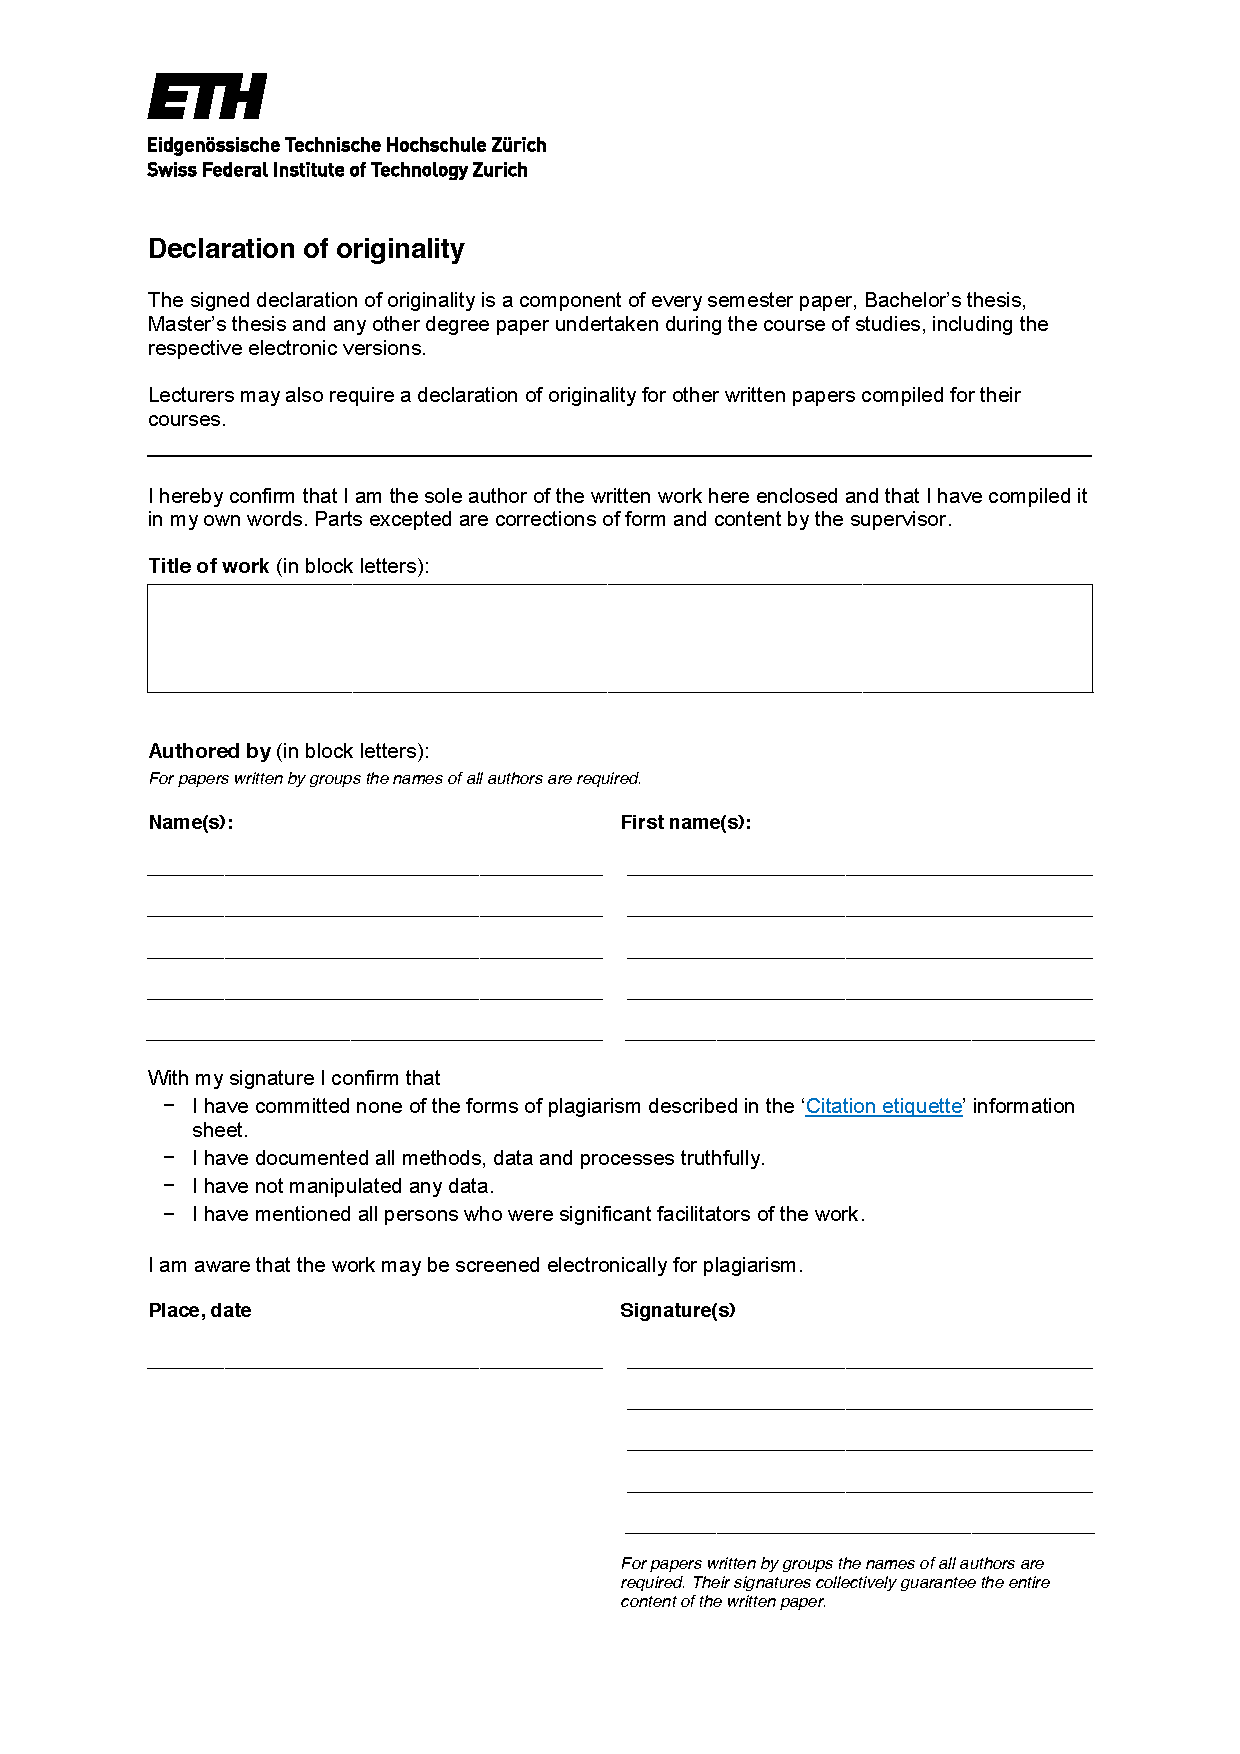
\includepdf[pages={-}]{declaration-originality.pdf}

\end{document}
